\chapter*{Oracle Apex}

\section{Langkah-Langkah membuat aplikasi menggunakan Apex}

Berikut langkah-langkah membuat aplikasi apex.
\begin{enumerate}
\item Buka website oracle apex dan klik sign in
\begin{figure}[H]
        \centerline{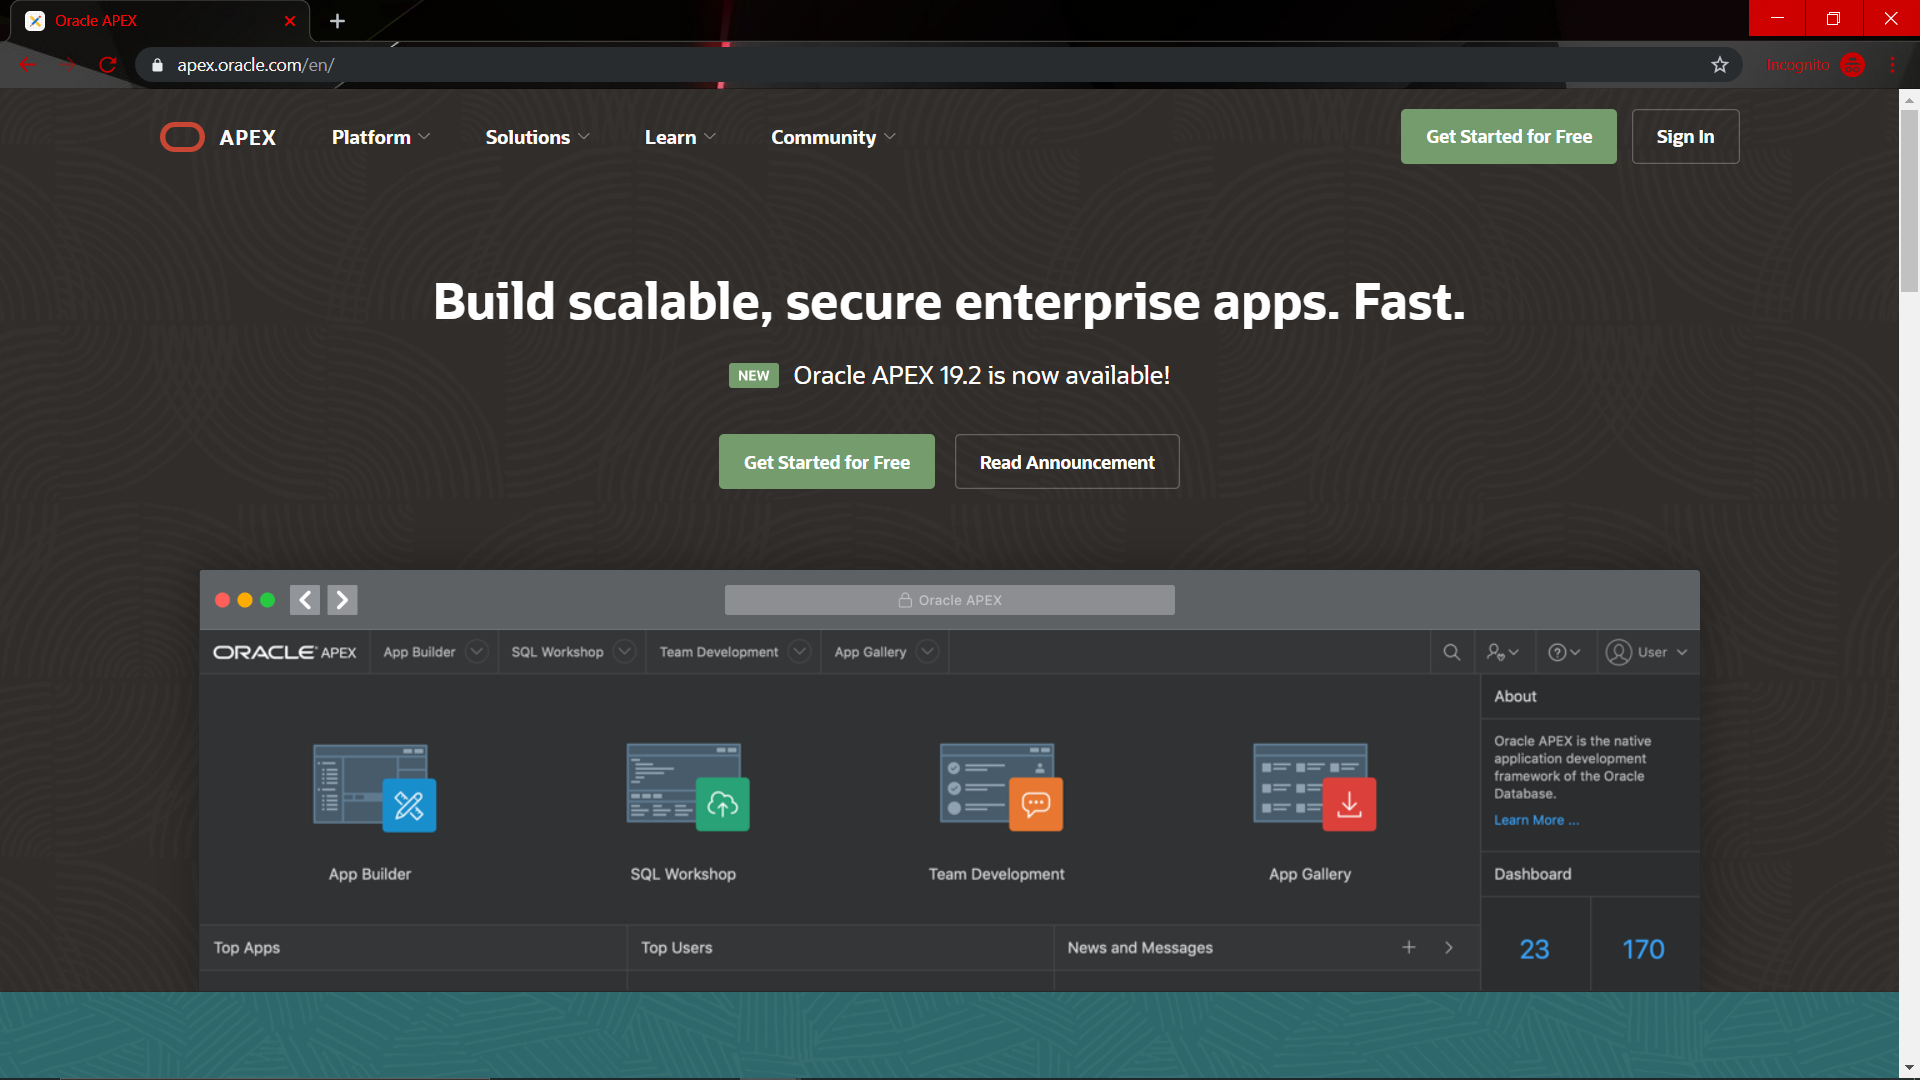
\includegraphics[scale=0.1]{figures/1}}
        \caption{}
		\label{langkah1}
\end{figure}

\item klik request workspace
\begin{figure}[H]
        \centerline{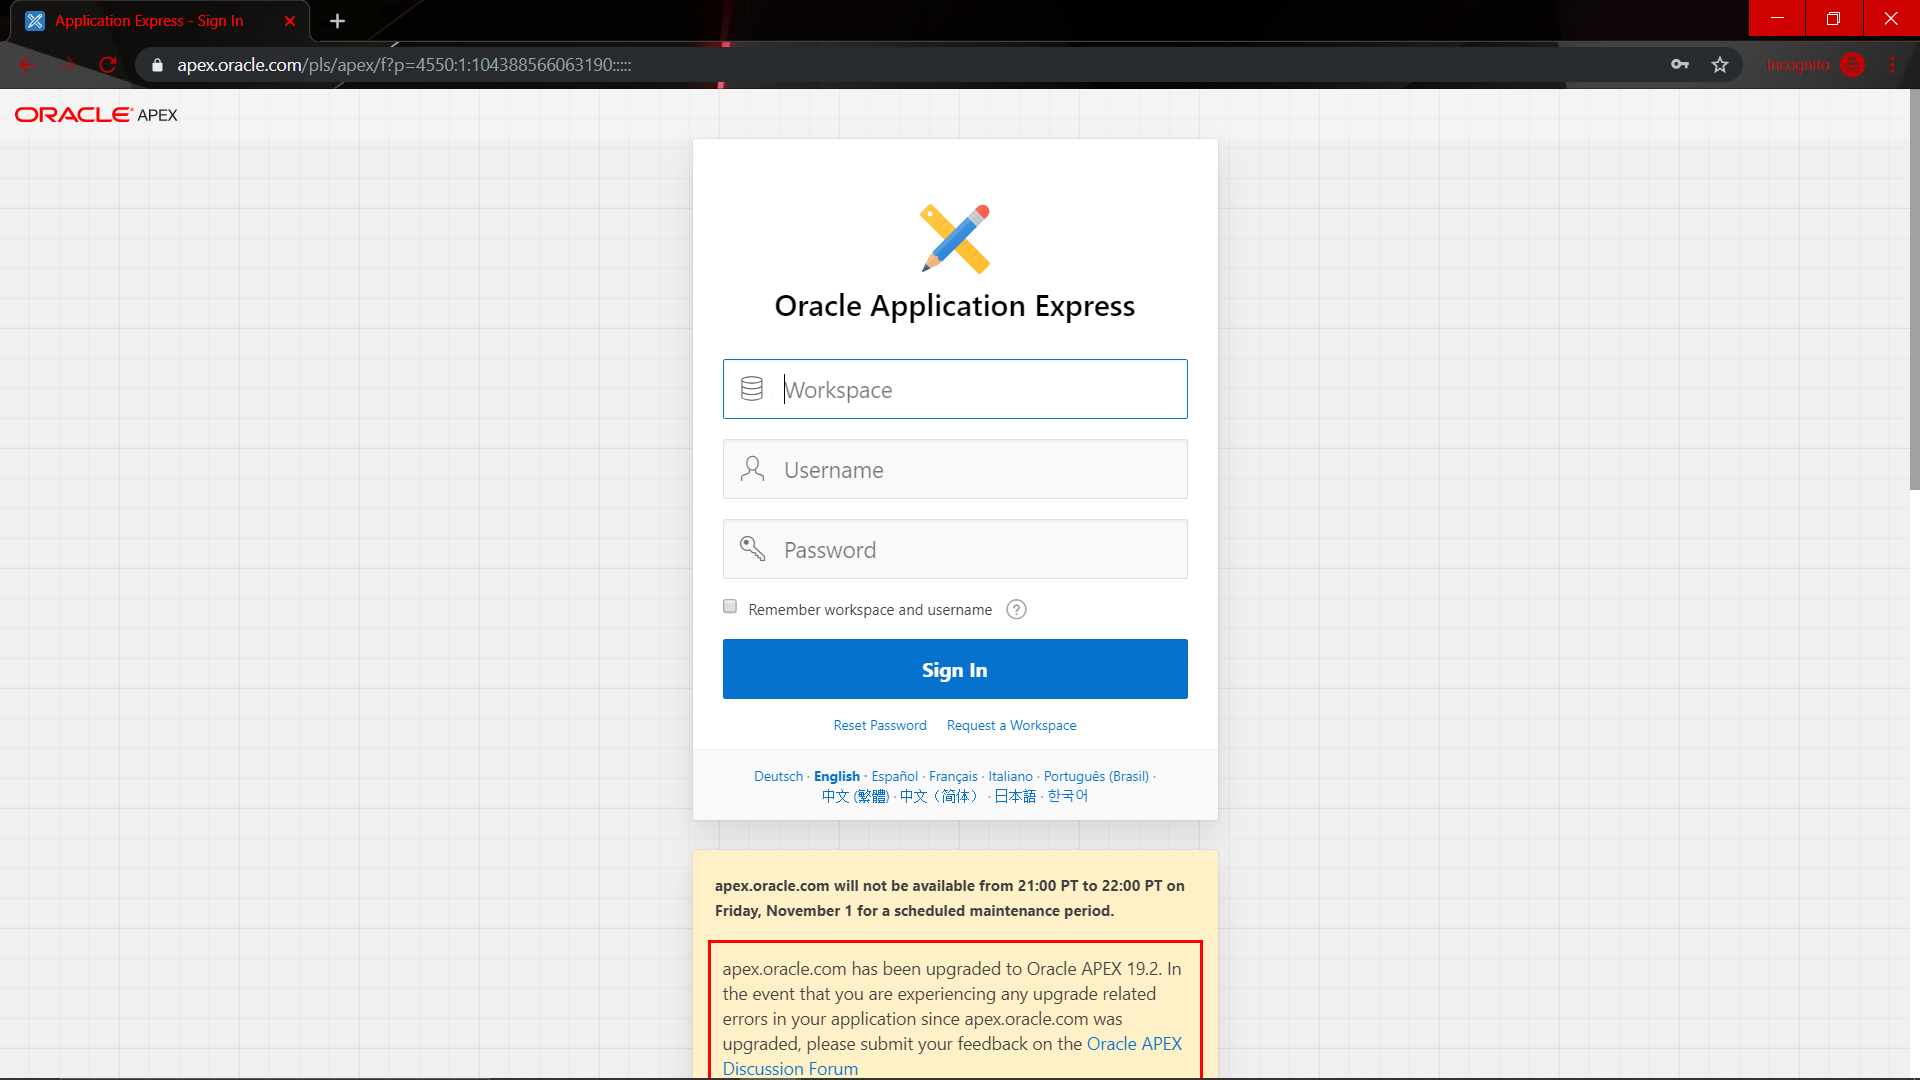
\includegraphics[scale=0.1]{figures/2}}
        \caption{}
		\label{langkah2}
\end{figure}


\item isi request workspace
\begin{figure}[H]
        \centerline{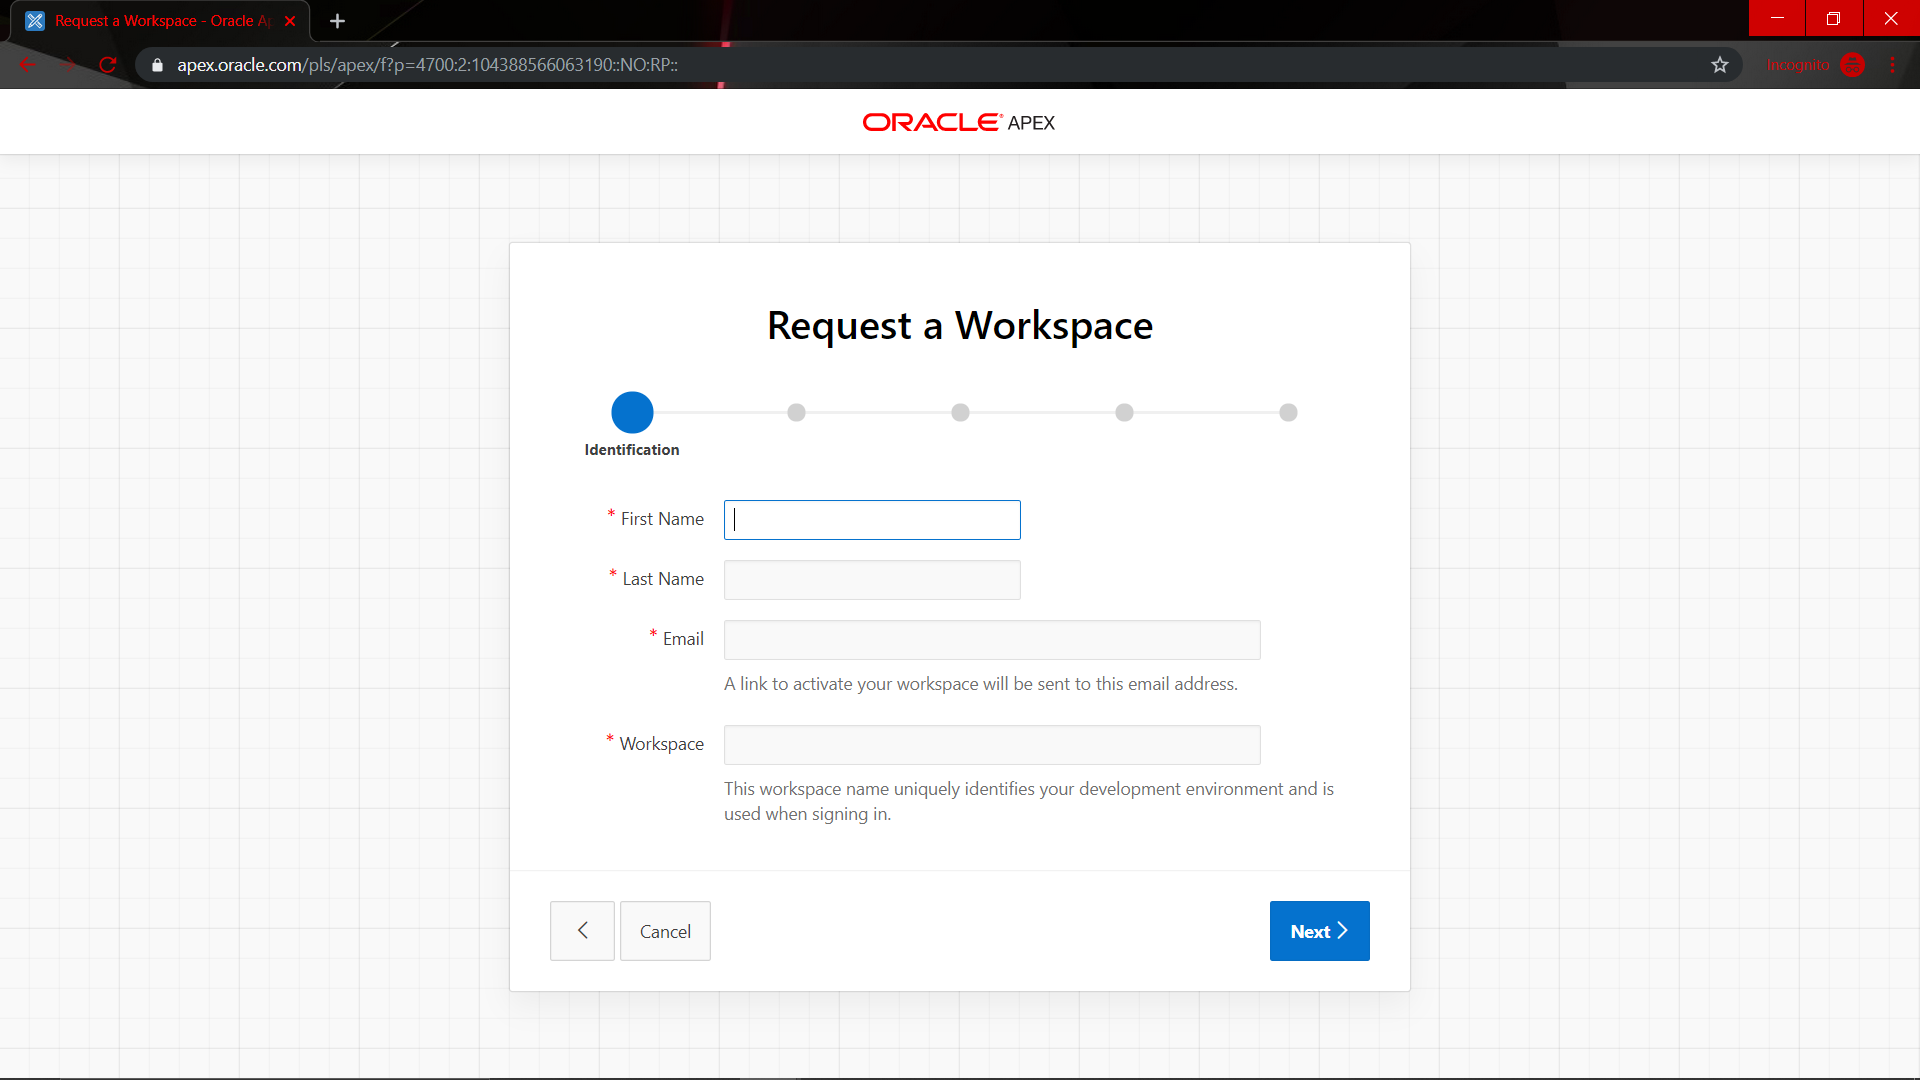
\includegraphics[scale=0.1]{figures/3}}
        \caption{}
		\label{langkah2}
\end{figure}


\item isi survey

\begin{figure}[H]
    \centering
    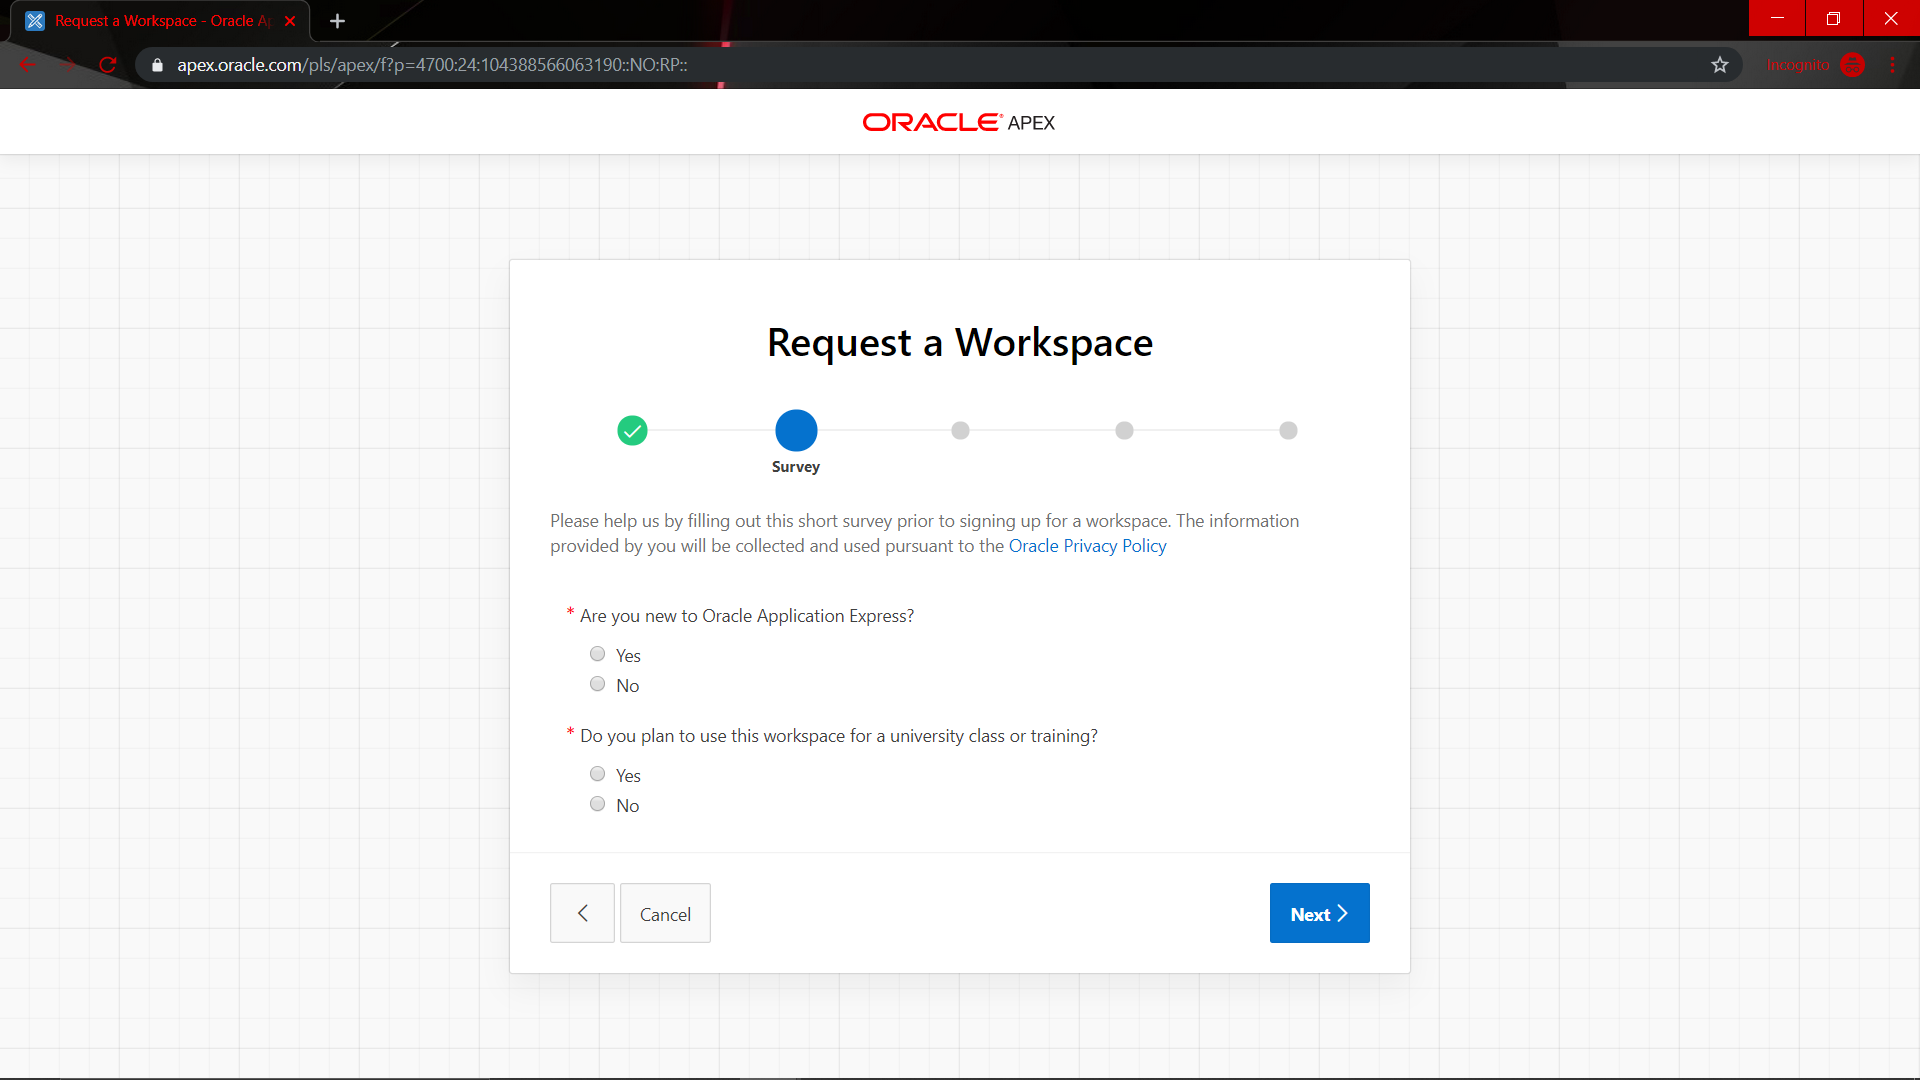
\includegraphics[scale=0.1]{figures/4}
    \caption{}
    \label{Figureanaconda3}
\end{figure}


\item isi justification

\begin{figure}[H]
    \centering
    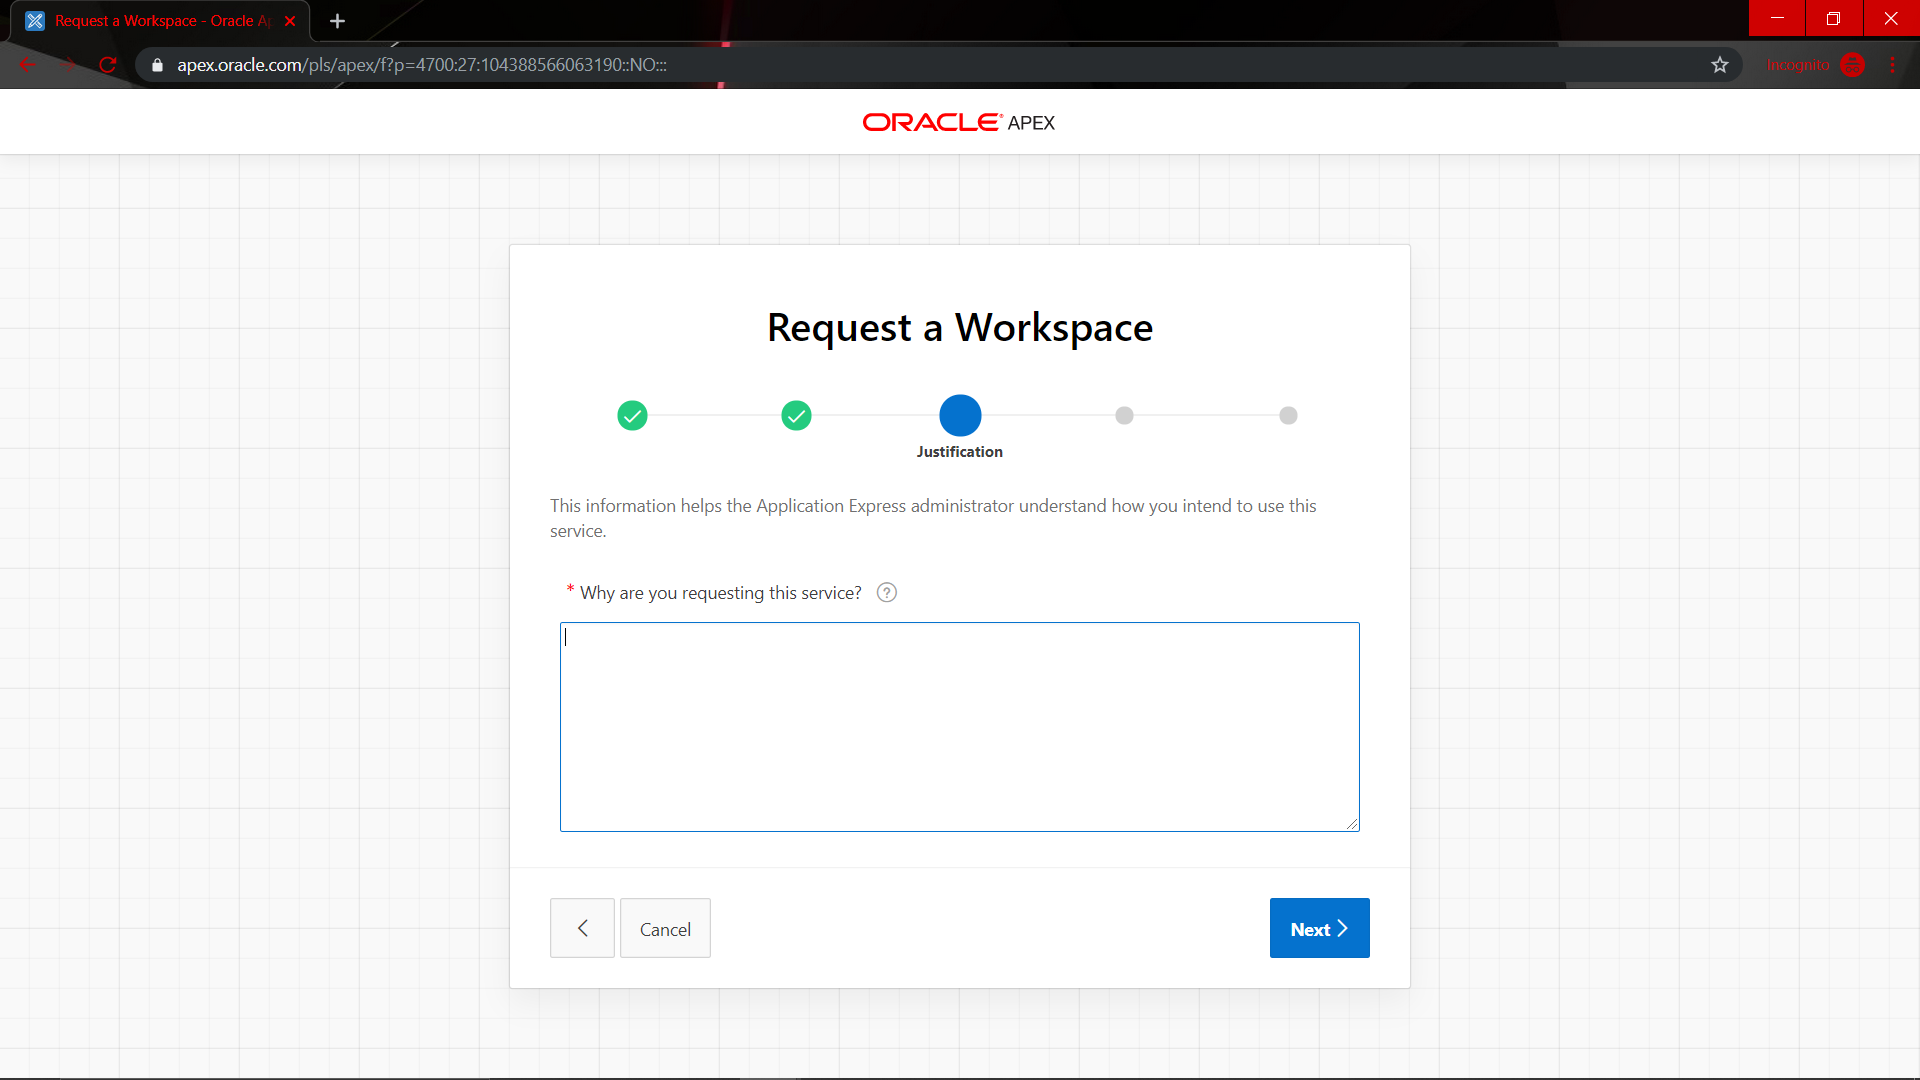
\includegraphics[scale=0.1]{figures/5}
    \caption{}
    \label{Figureanaconda4}
\end{figure}


\item isi agreement

\begin{figure}[H]
    \centering
    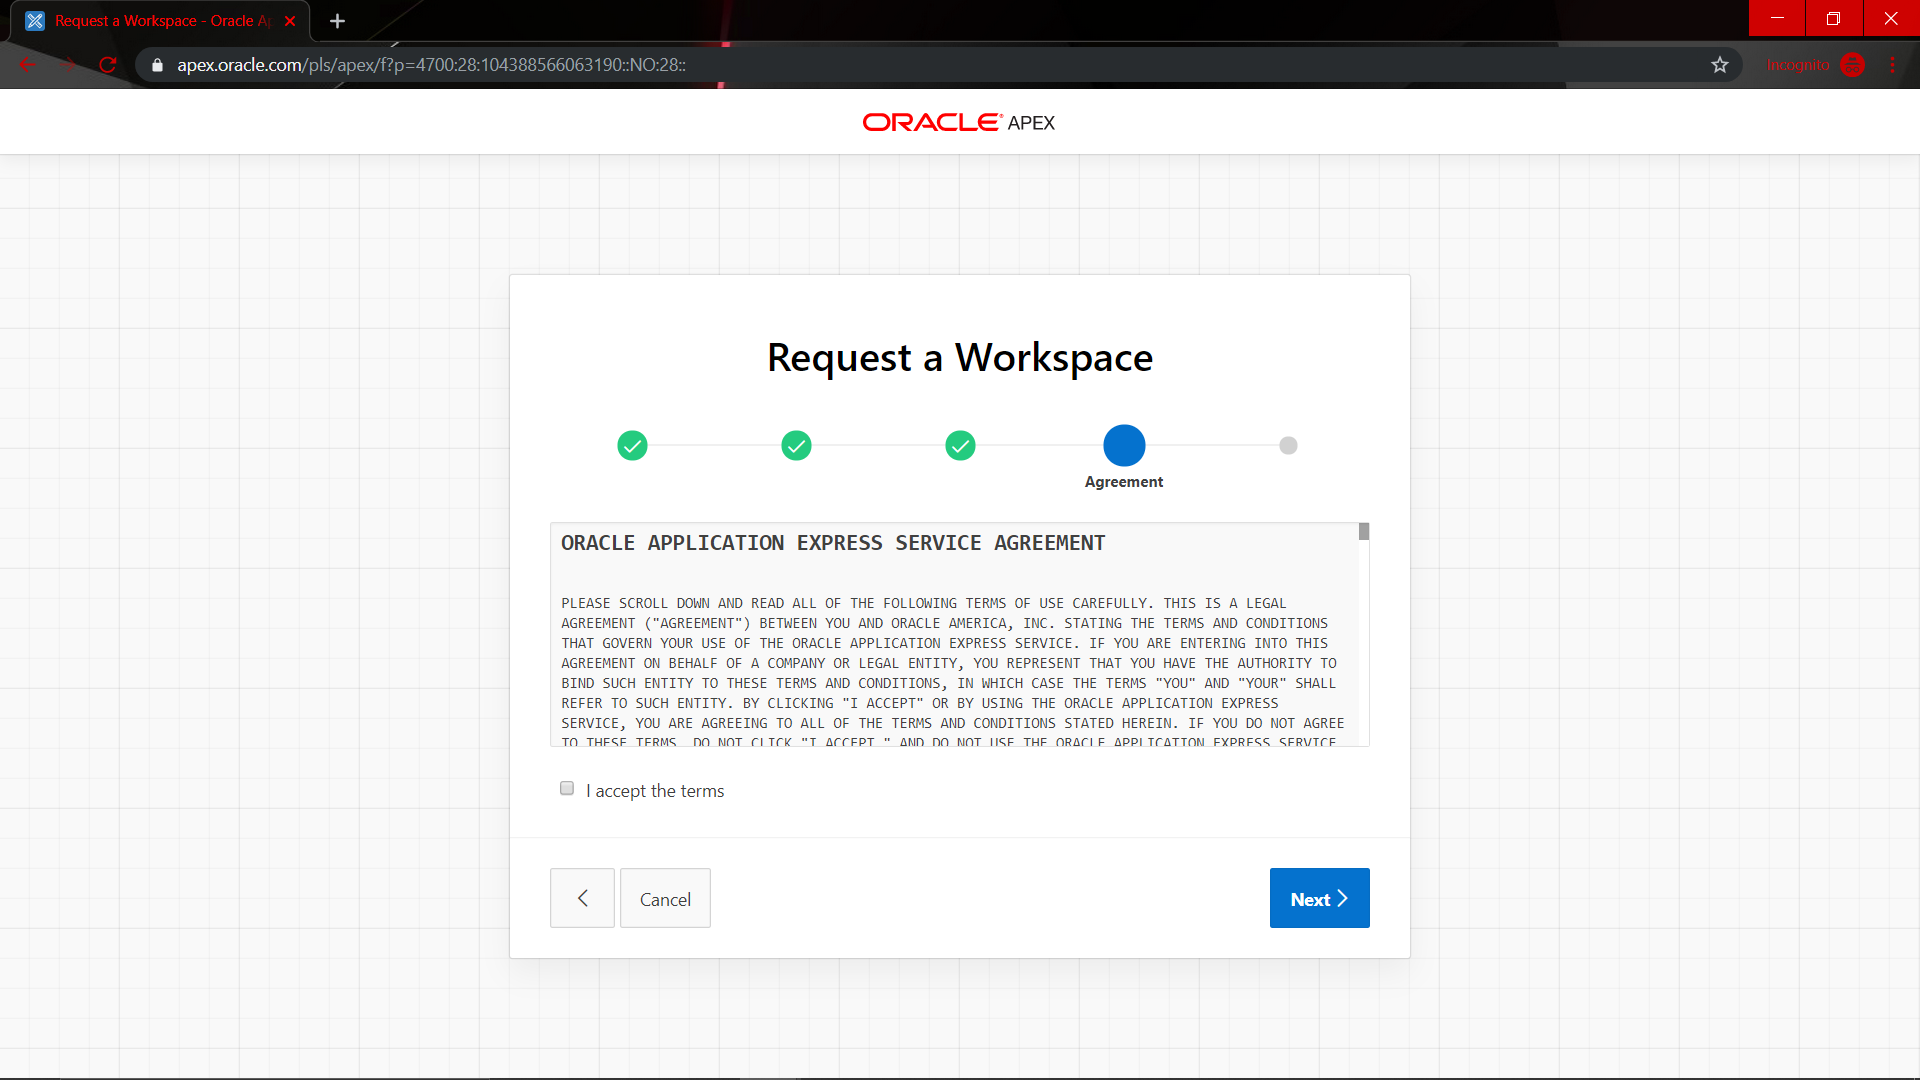
\includegraphics[scale=0.1]{figures/6}
    \caption{}
    \label{Figureanaconda5}
\end{figure}


\item buka email dan buka email dari oracle karena workspace di approved oleh oracle lalu klik create workspace
\begin{figure}[H]
    \centering
    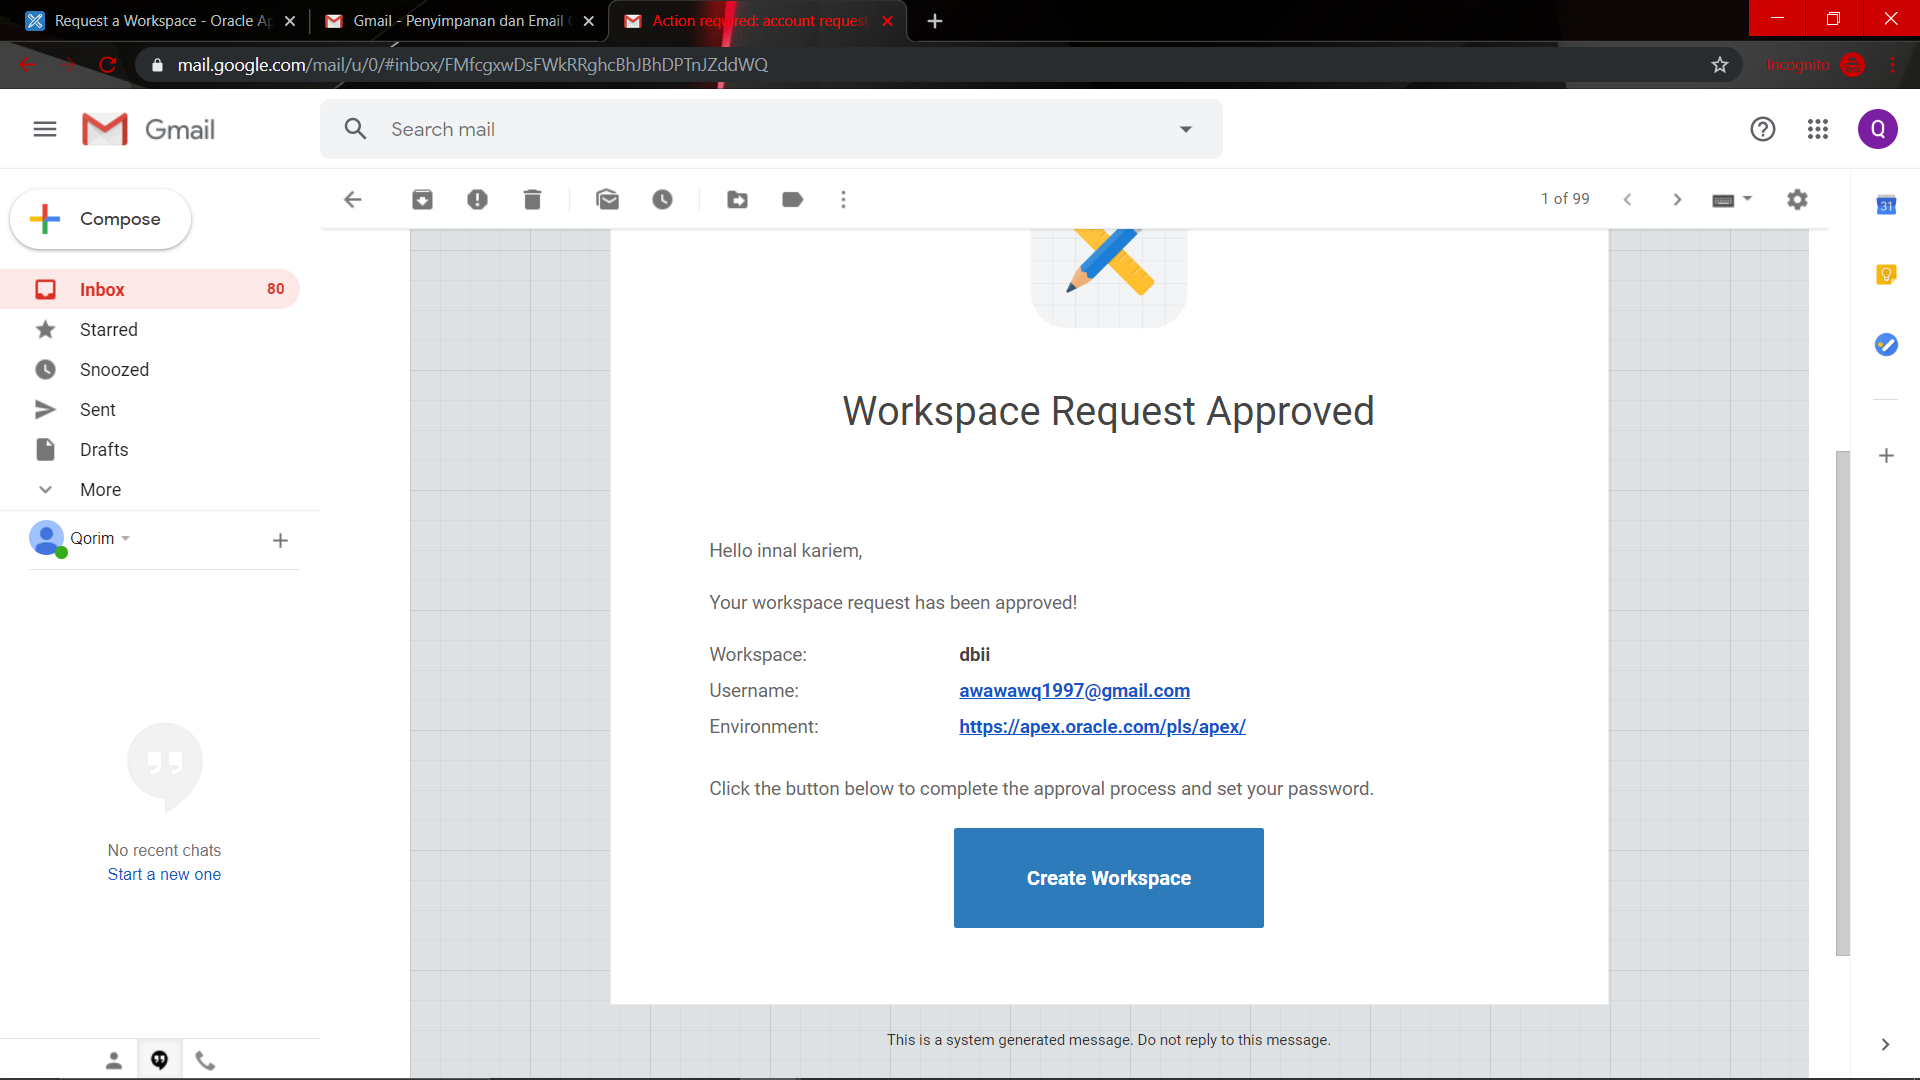
\includegraphics[scale=0.1]{figures/7}
    \caption{}
    \label{Figureanaconda6}
\end{figure}

\item setelah itu akan masuk ke apexnya, lalu masukan password untuk workspace tersebut

\begin{figure}[H]
    \centering
    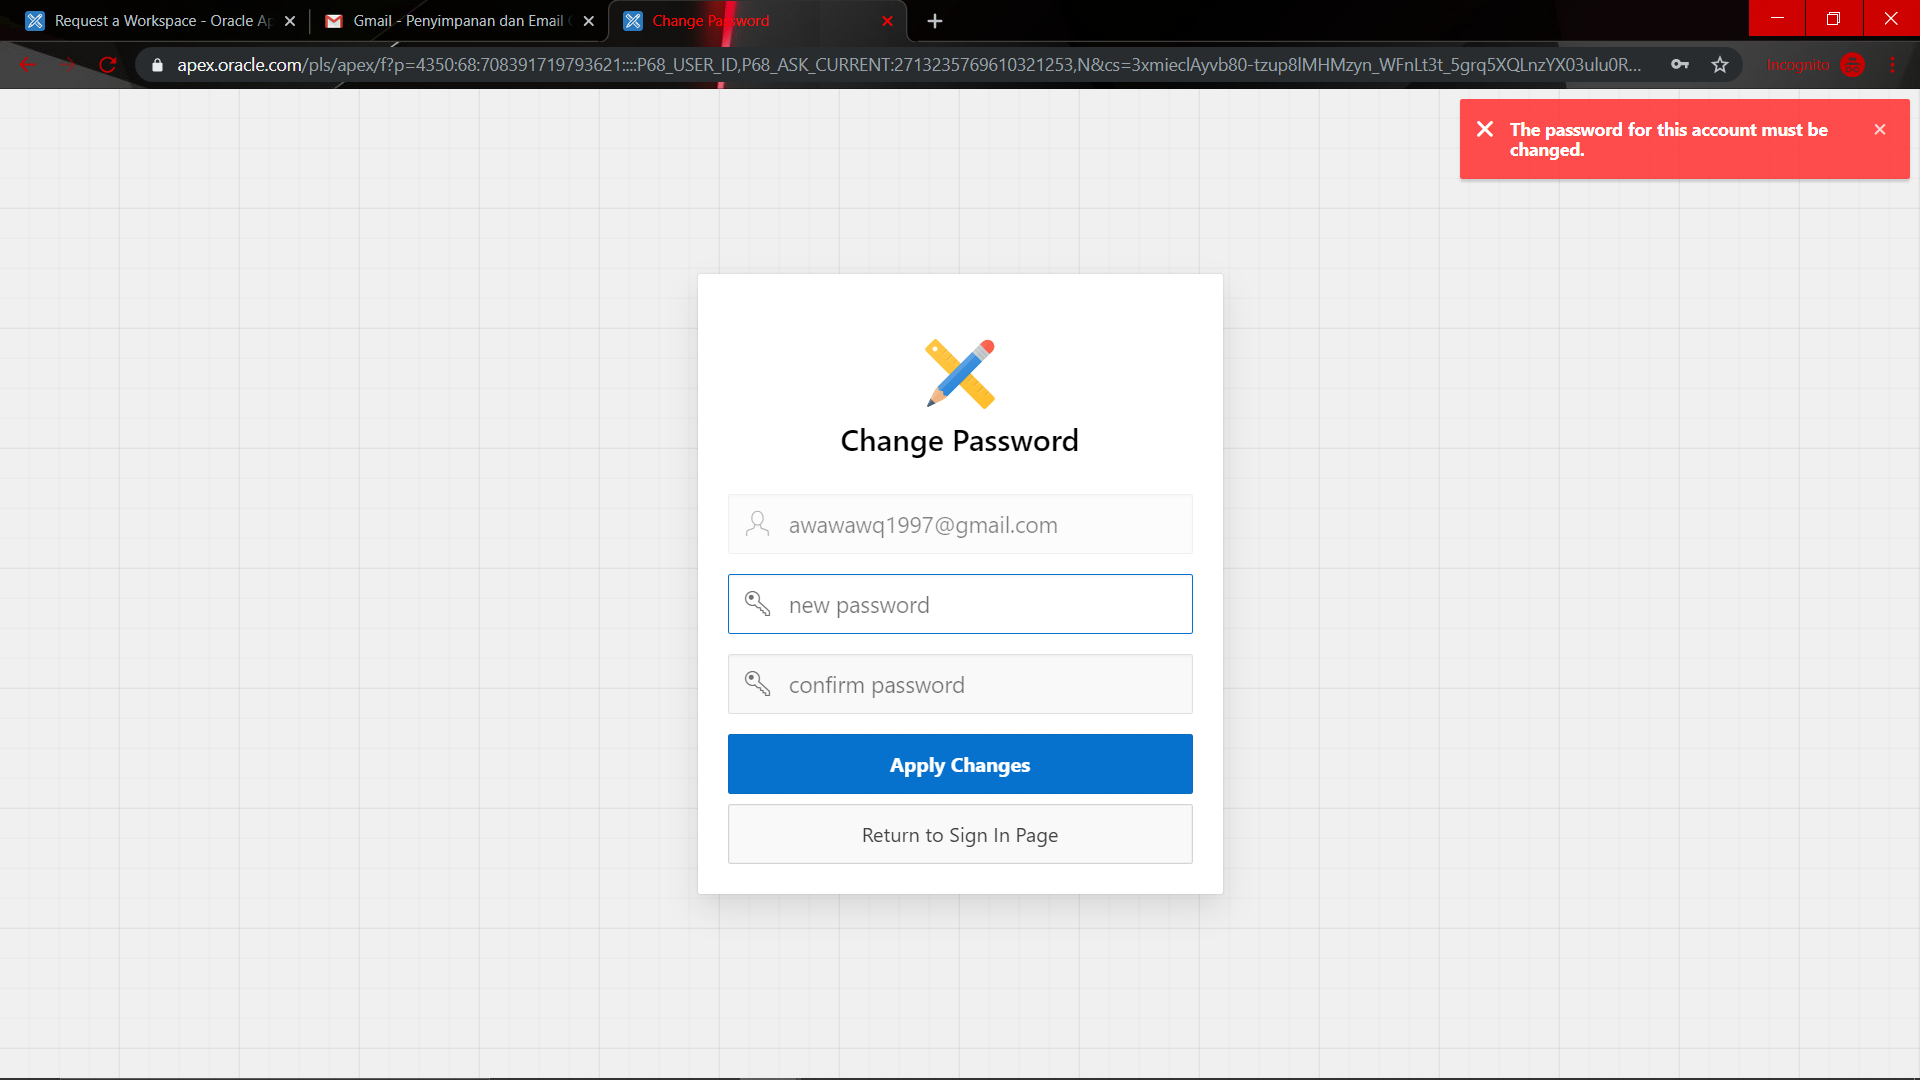
\includegraphics[scale=0.1]{figures/8}
    \caption{}
    \label{Figureanaconda7}
\end{figure}

\item klik app builder
\begin{figure}[H]
    \centering
    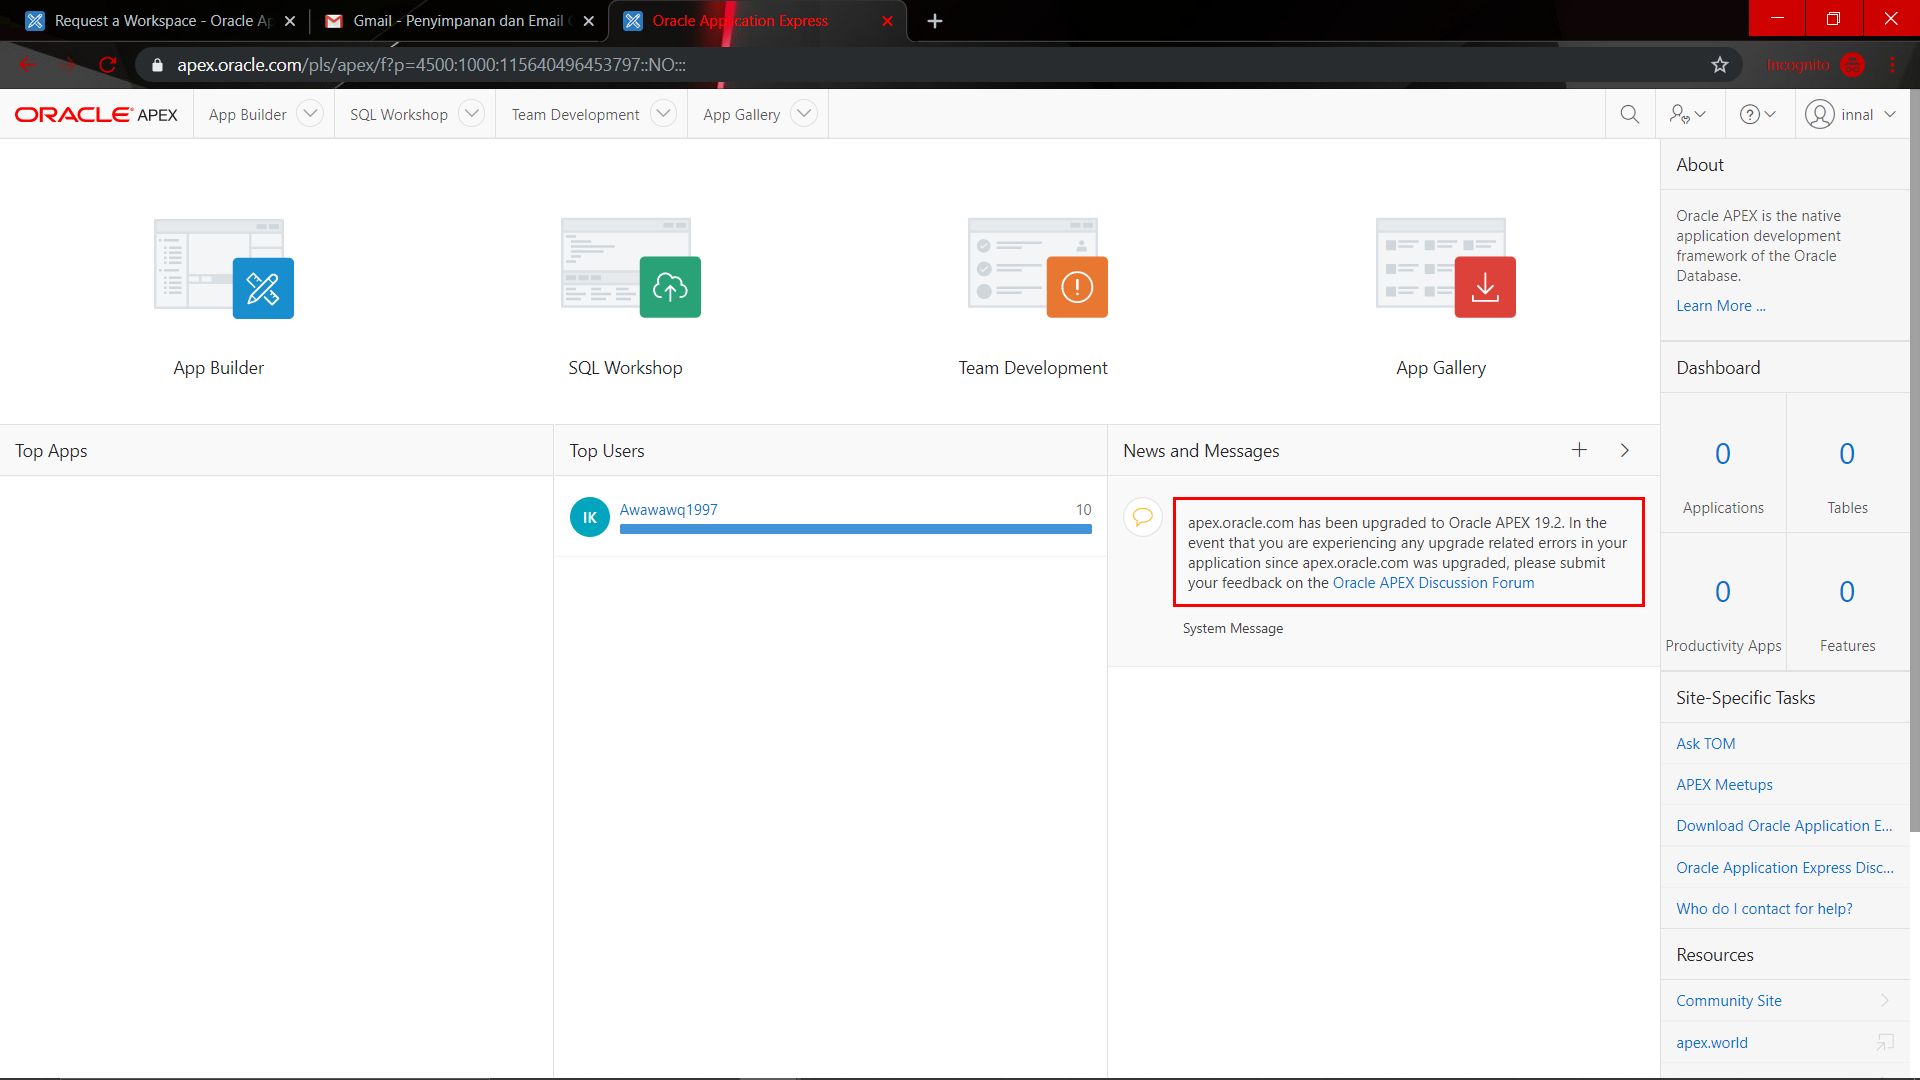
\includegraphics[scale=0.1]{figures/9}
    \caption{}
    \label{Figureanaconda8}
\end{figure}

\item klik create 
\begin{figure}[H]
    \centering
    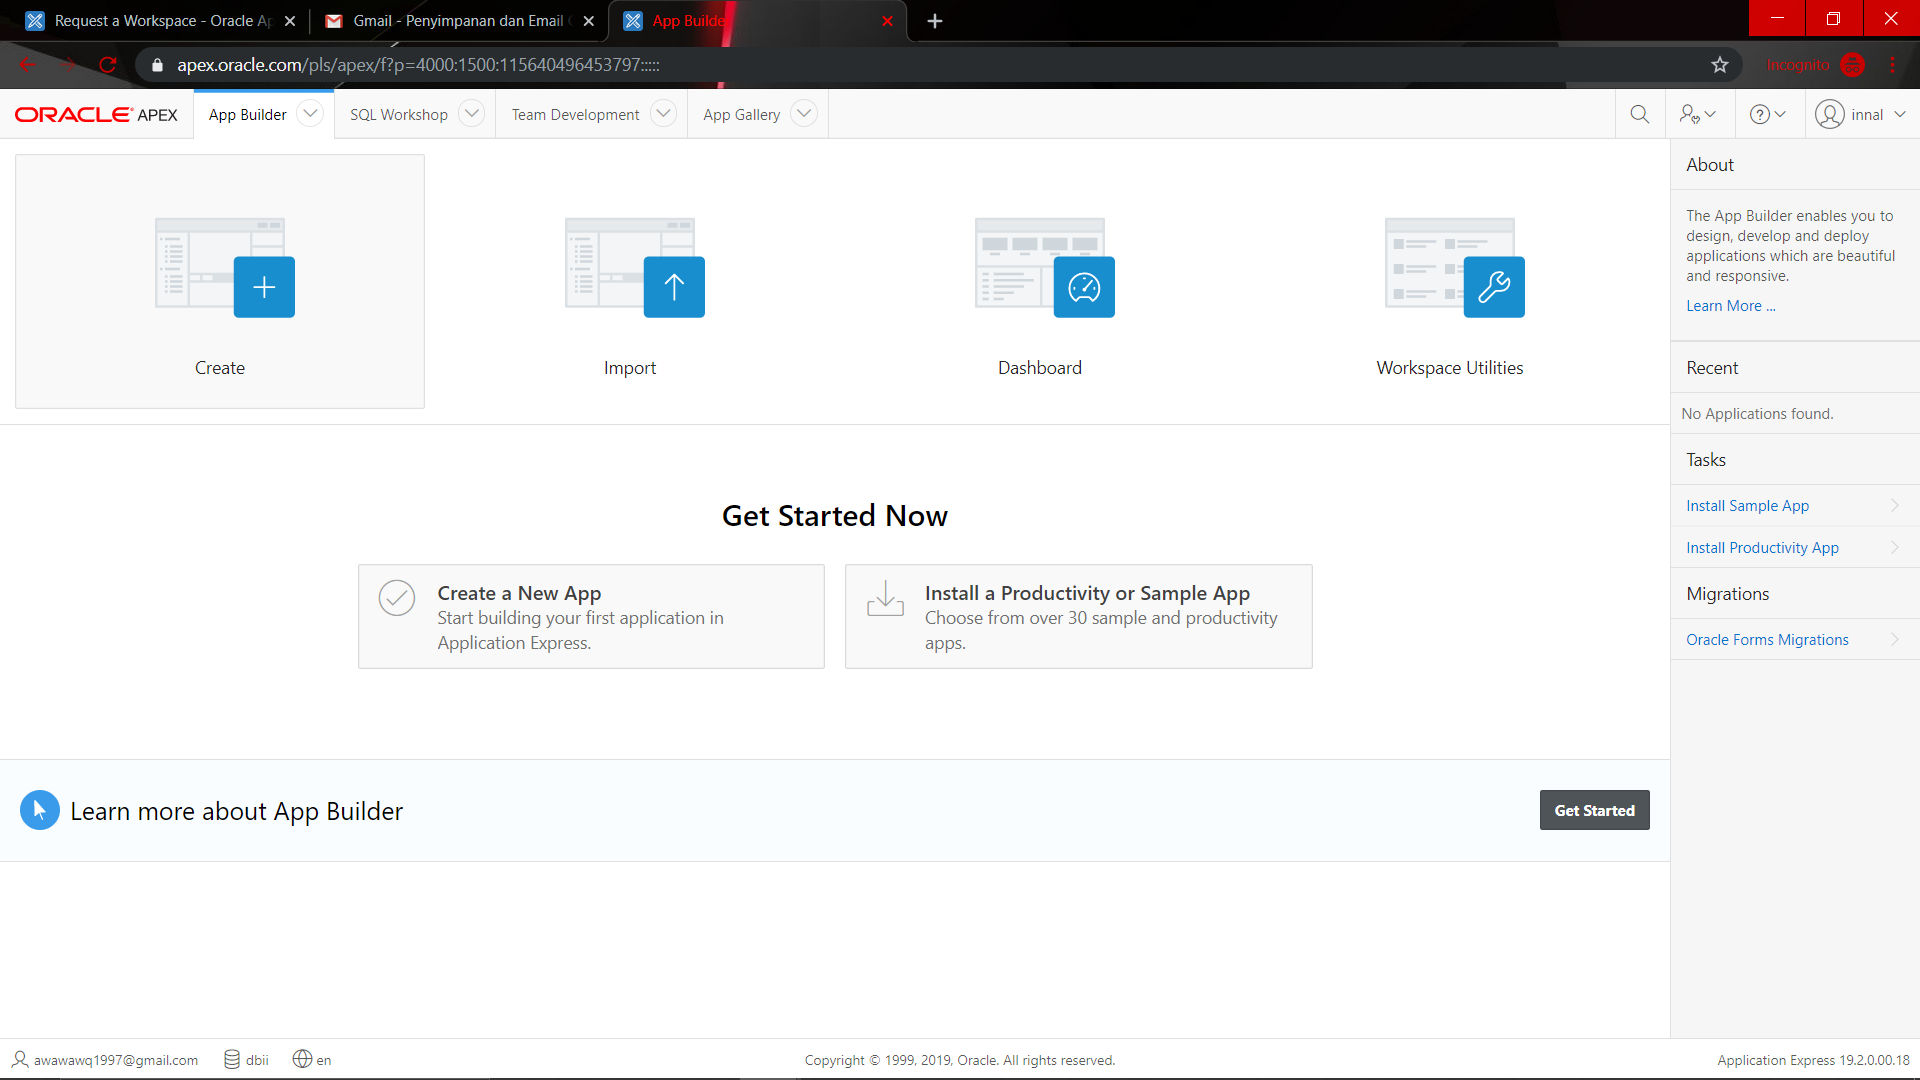
\includegraphics[scale=0.1]{figures/10}
    \caption{}
    \label{Figureanaconda70}
\end{figure}

\item klik from a file

\begin{figure}[H]
    \centering
    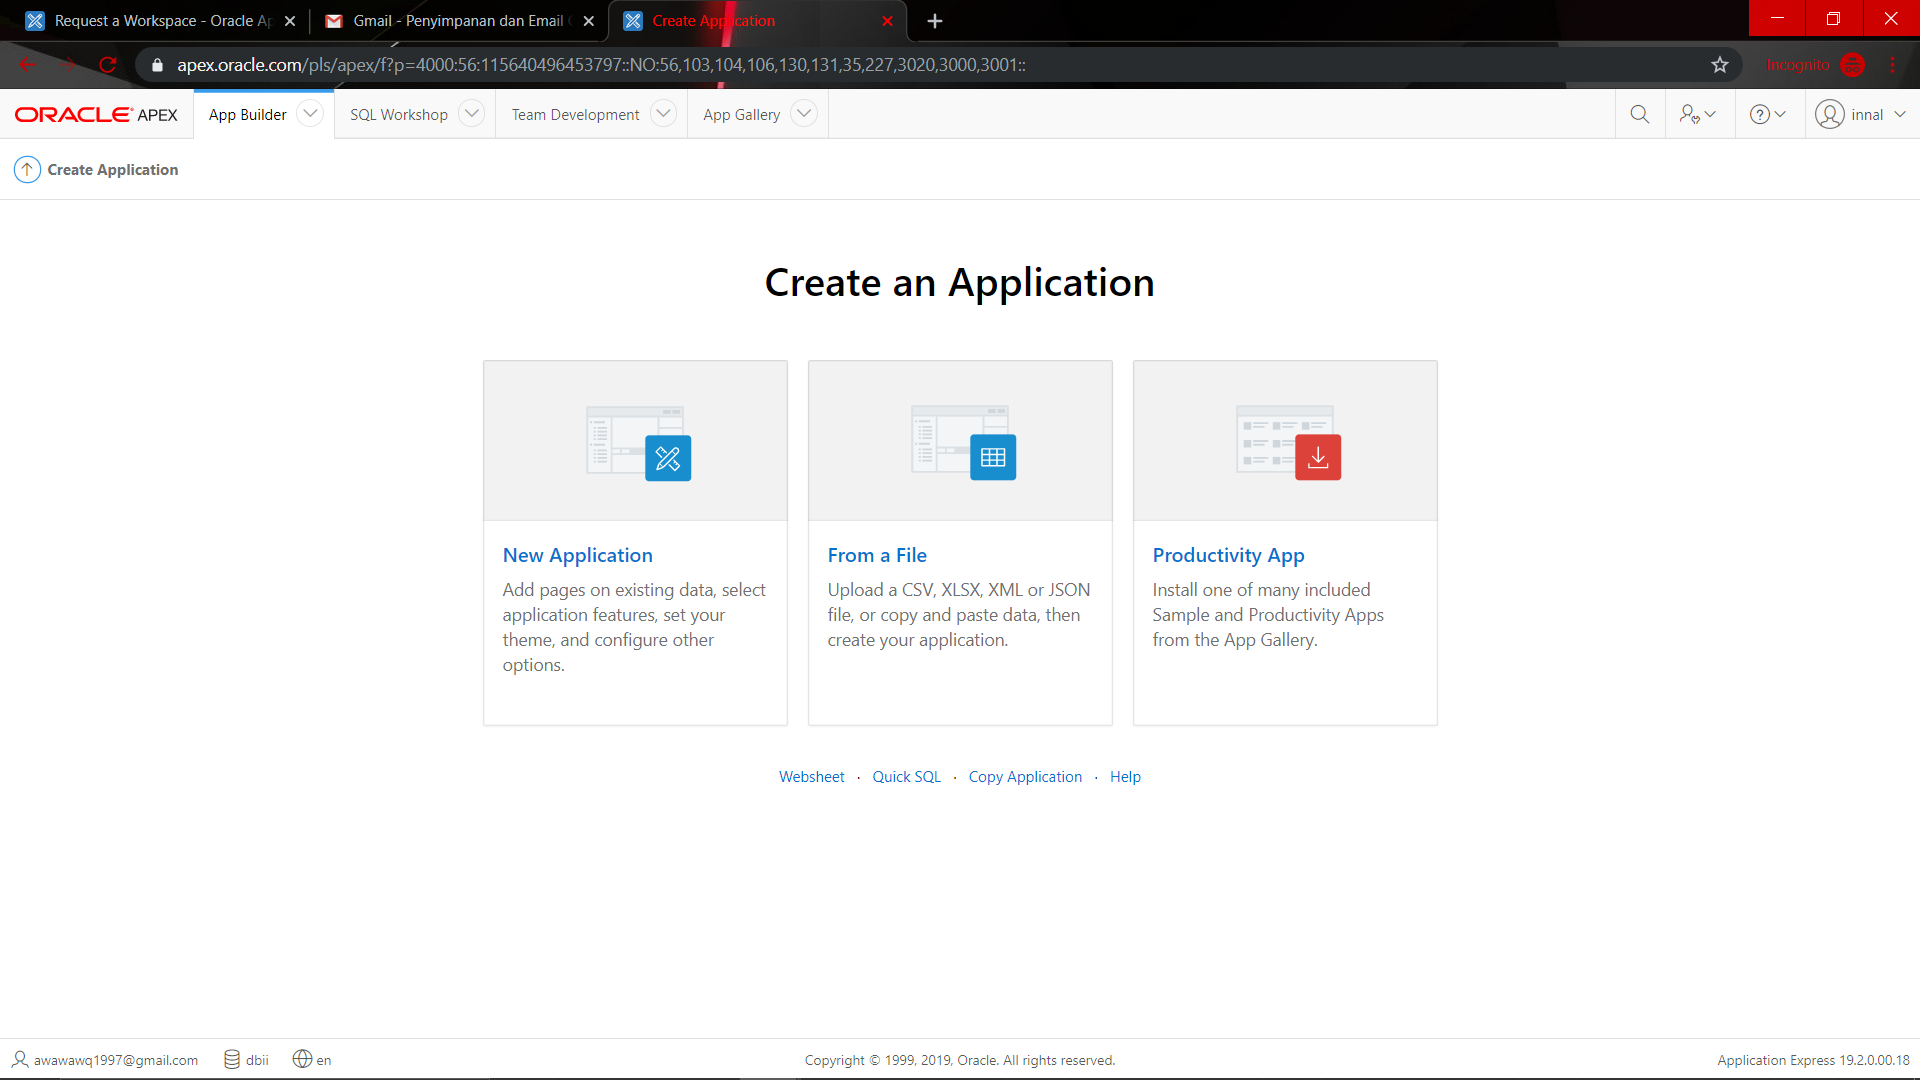
\includegraphics[scale=0.1]{figures/11}
    \caption{}
    \label{Figureanaconda70}
\end{figure}
\item masukan file 

\begin{figure}[H]
    \centering
    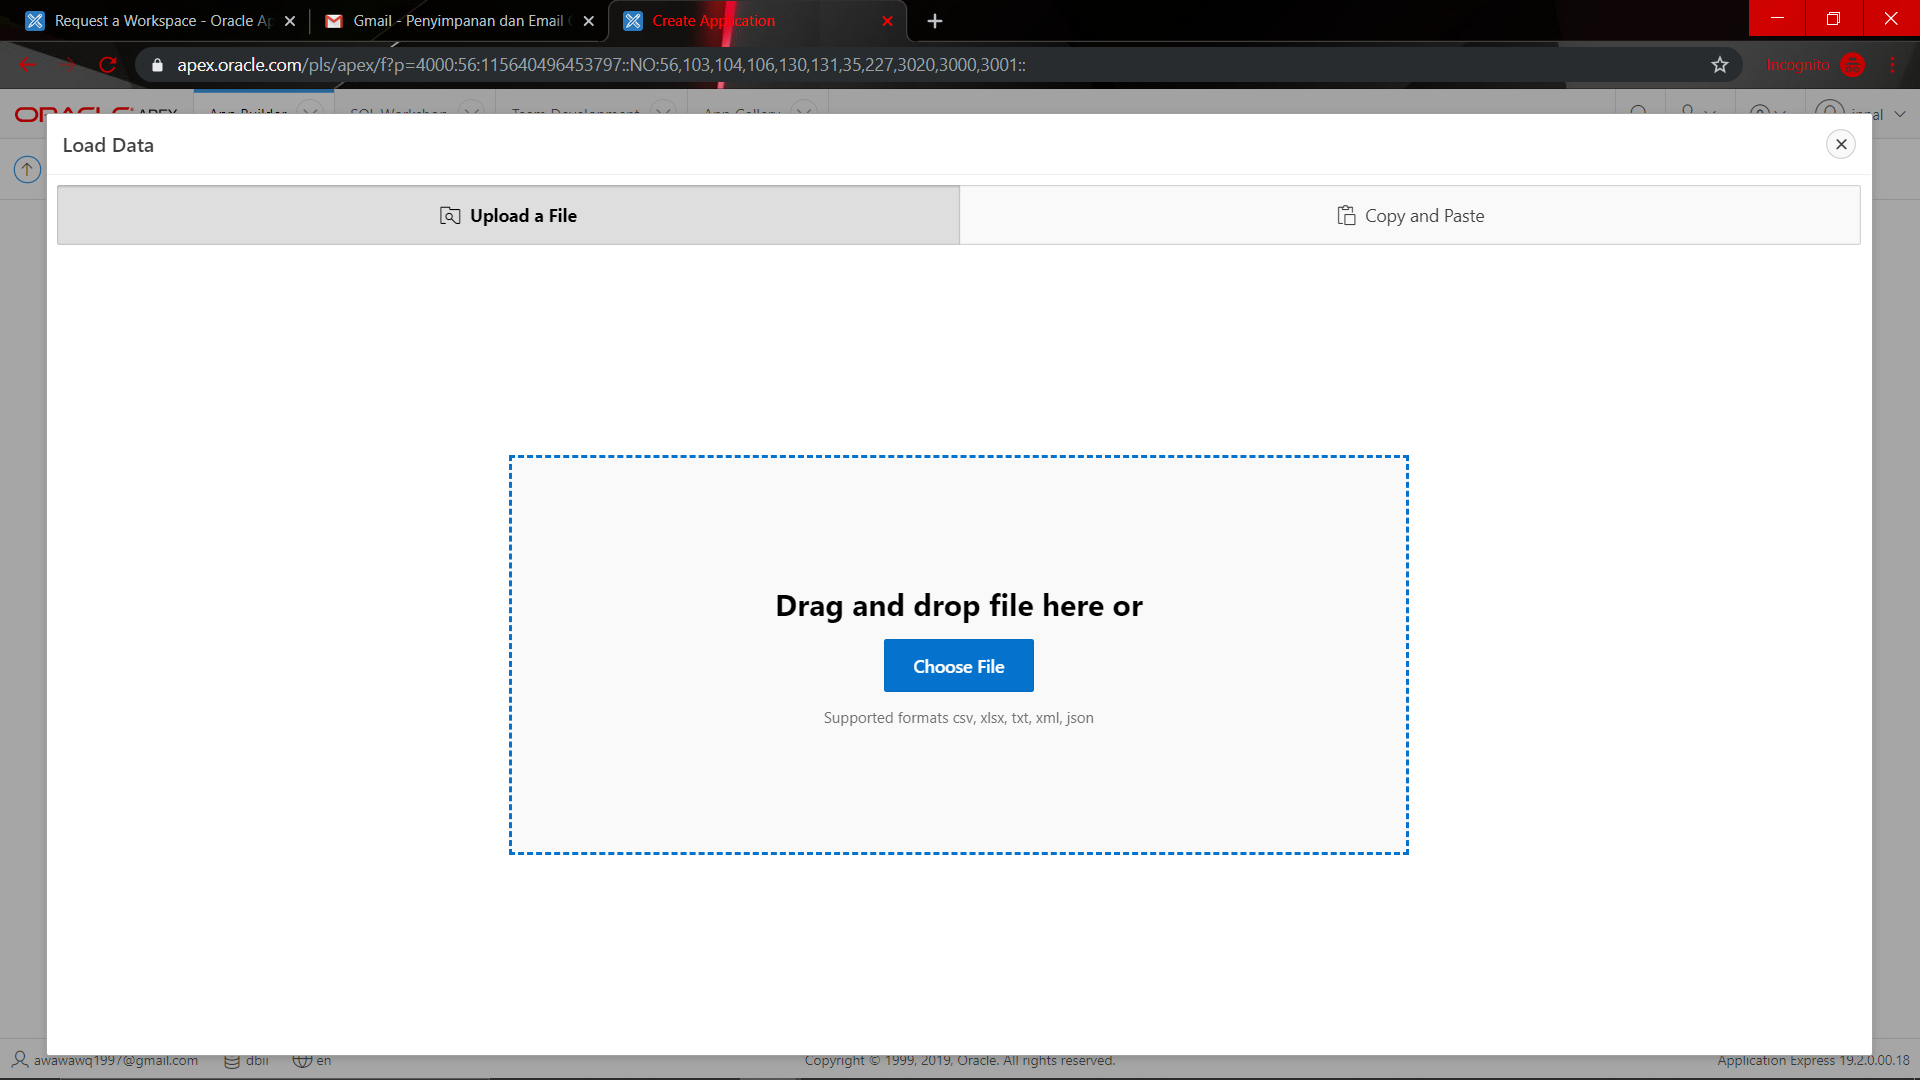
\includegraphics[scale=0.1]{figures/14}
    \caption{}
    \label{Figureanaconda70}
\end{figure}


\item berikan nama untuk file tersebut dan klik load data
\begin{figure}[H]
    \centering
    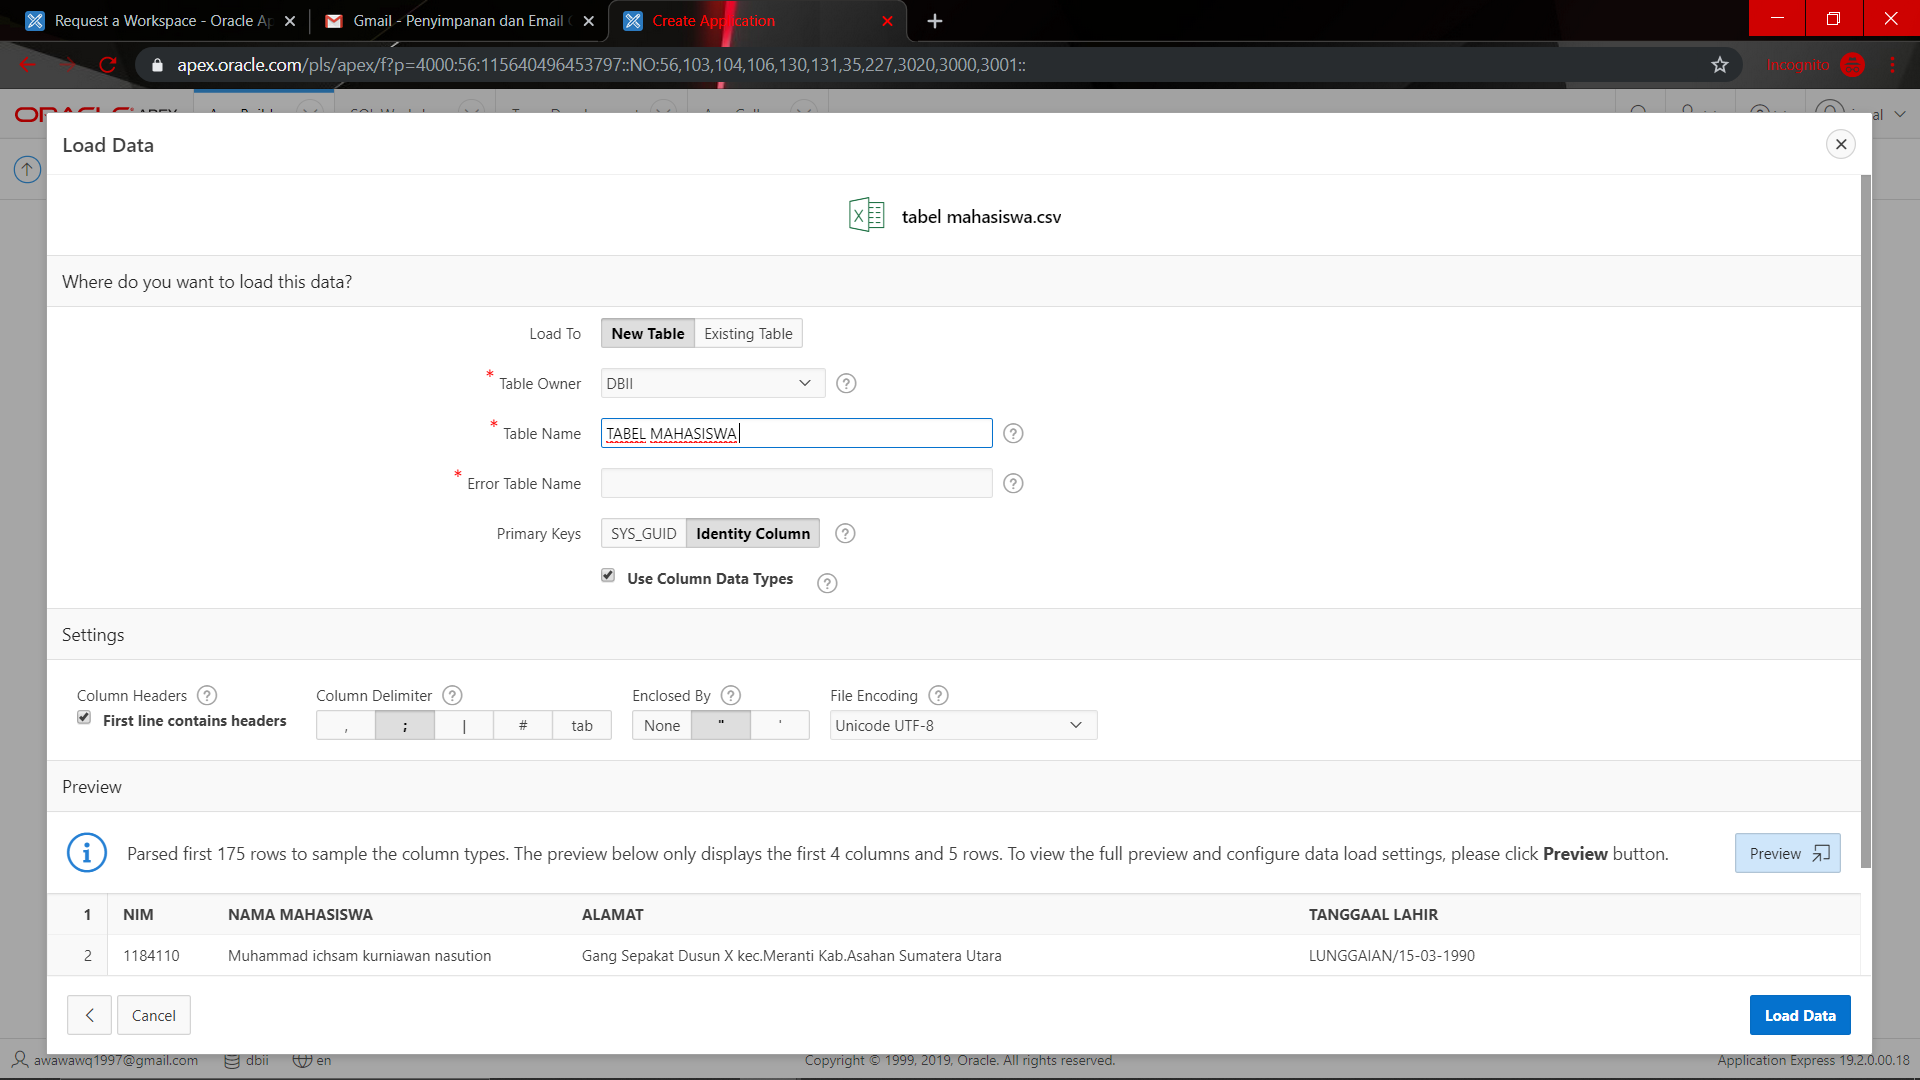
\includegraphics[scale=0.1]{figures/12}
    \caption{}
    \label{Figureanaconda70}
\end{figure}

\item klik from a file 
\begin{figure}[H]
    \centering
    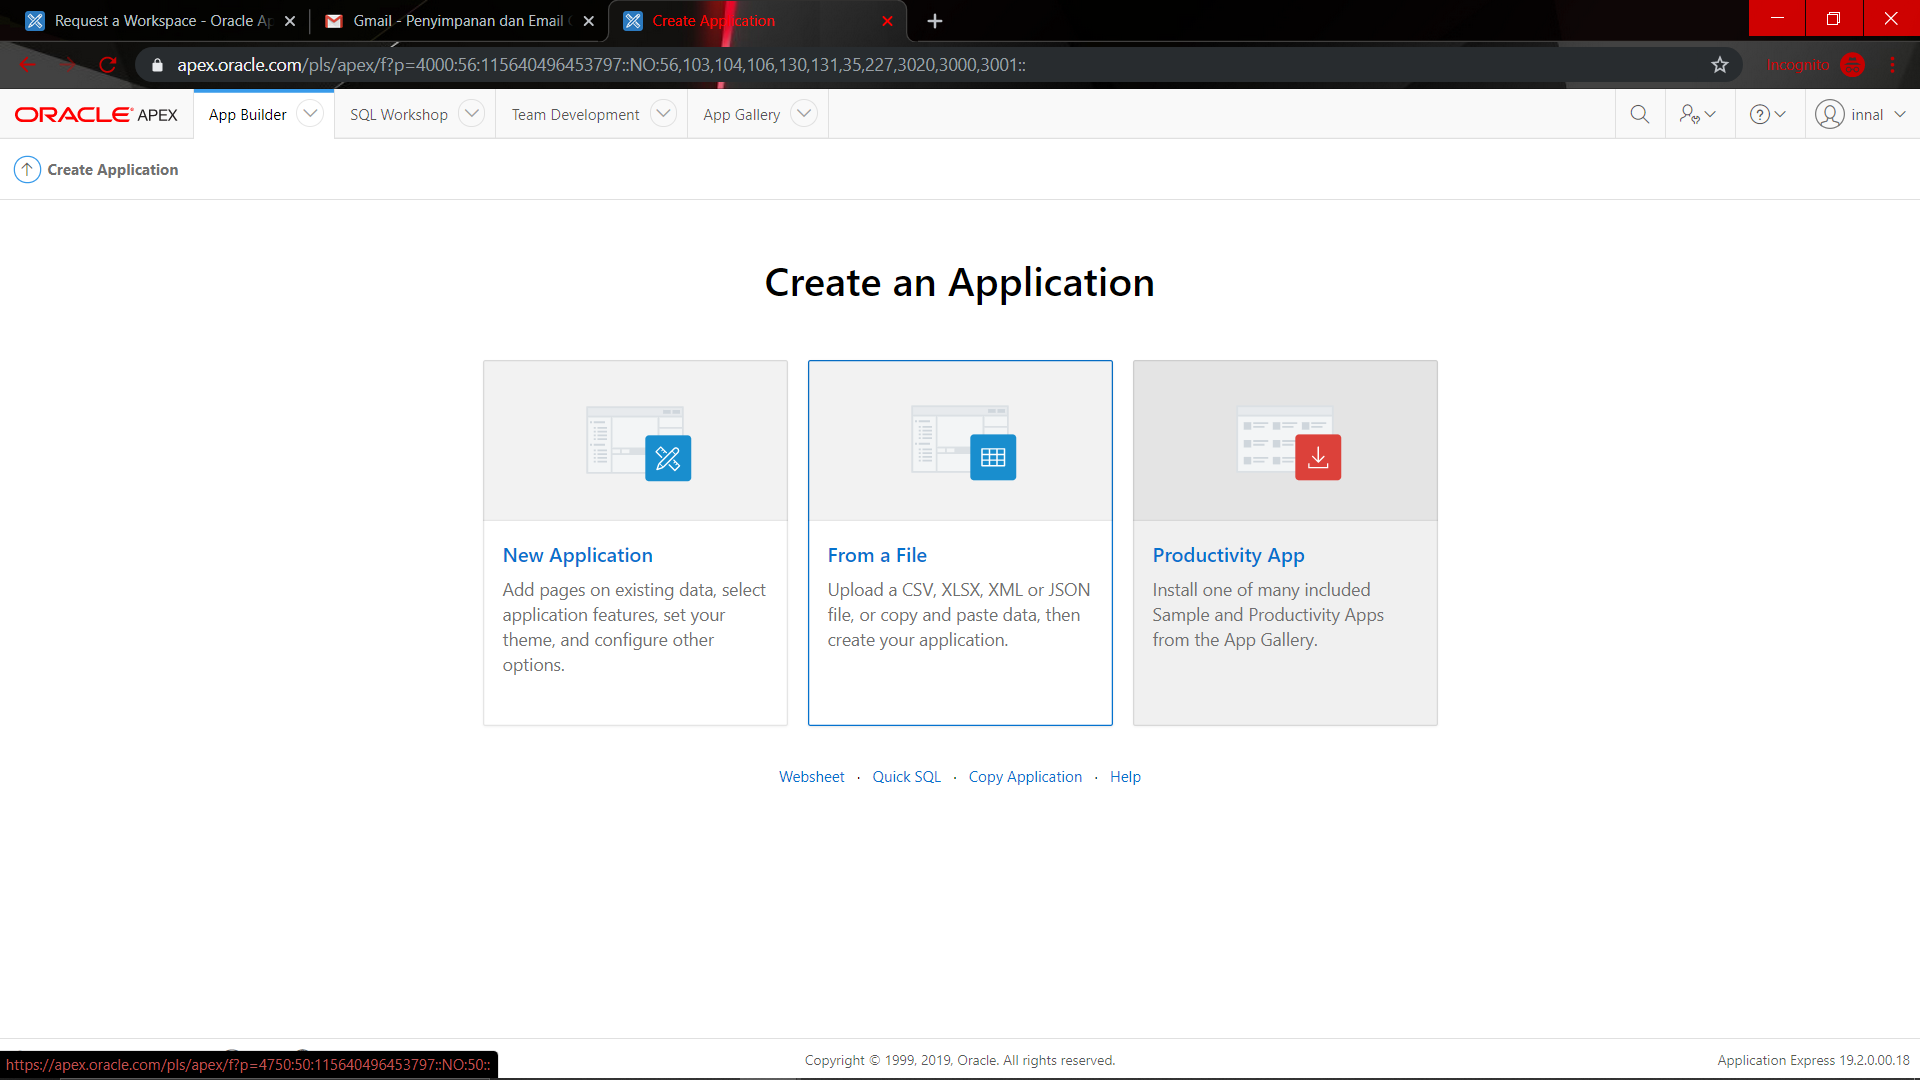
\includegraphics[scale=0.1]{figures/13}
    \caption{}
    \label{Figureanaconda70}
\end{figure}

\item masukan file lain yang ingin dimasukan 
\begin{figure}[H]
    \centering
    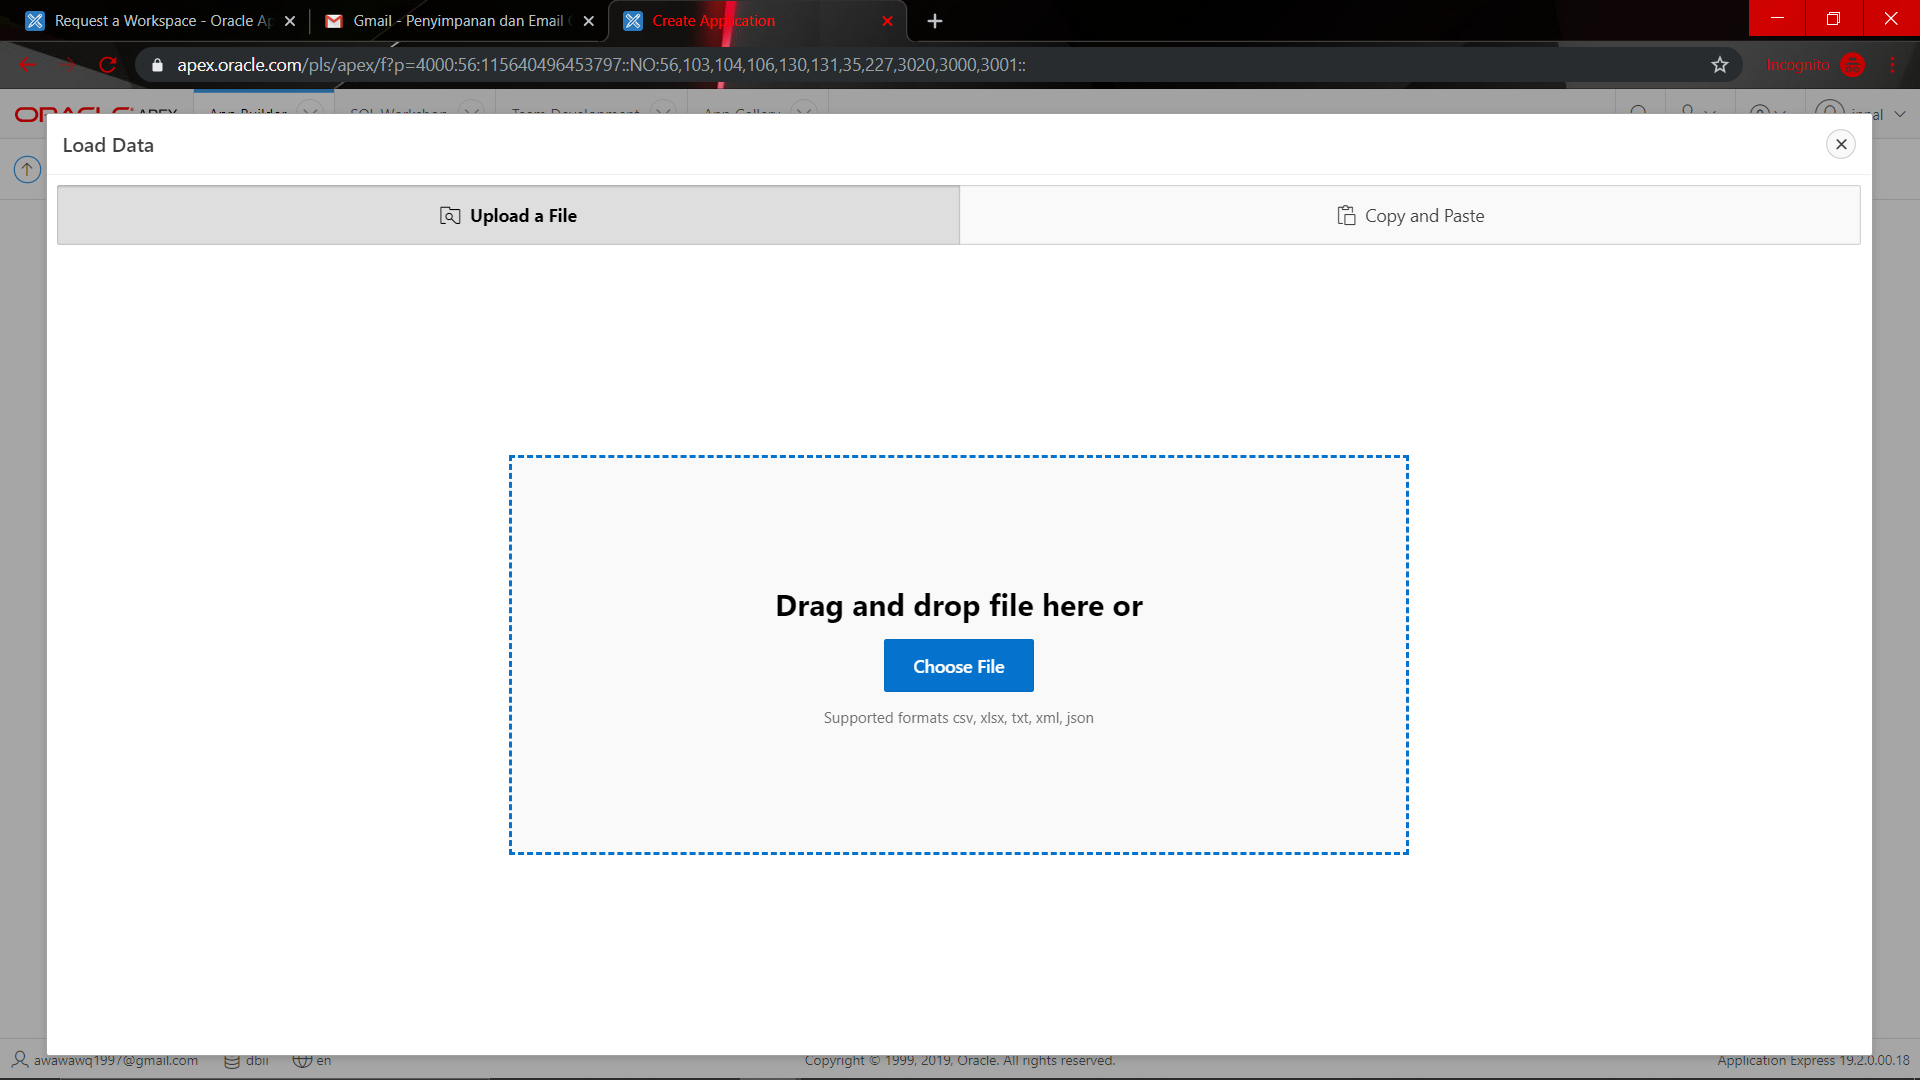
\includegraphics[scale=0.1]{figures/14}
    \caption{}
    \label{Figureanaconda70}
\end{figure}


\item berikan nama untuk file tersebut 
\begin{figure}[H]
    \centering
    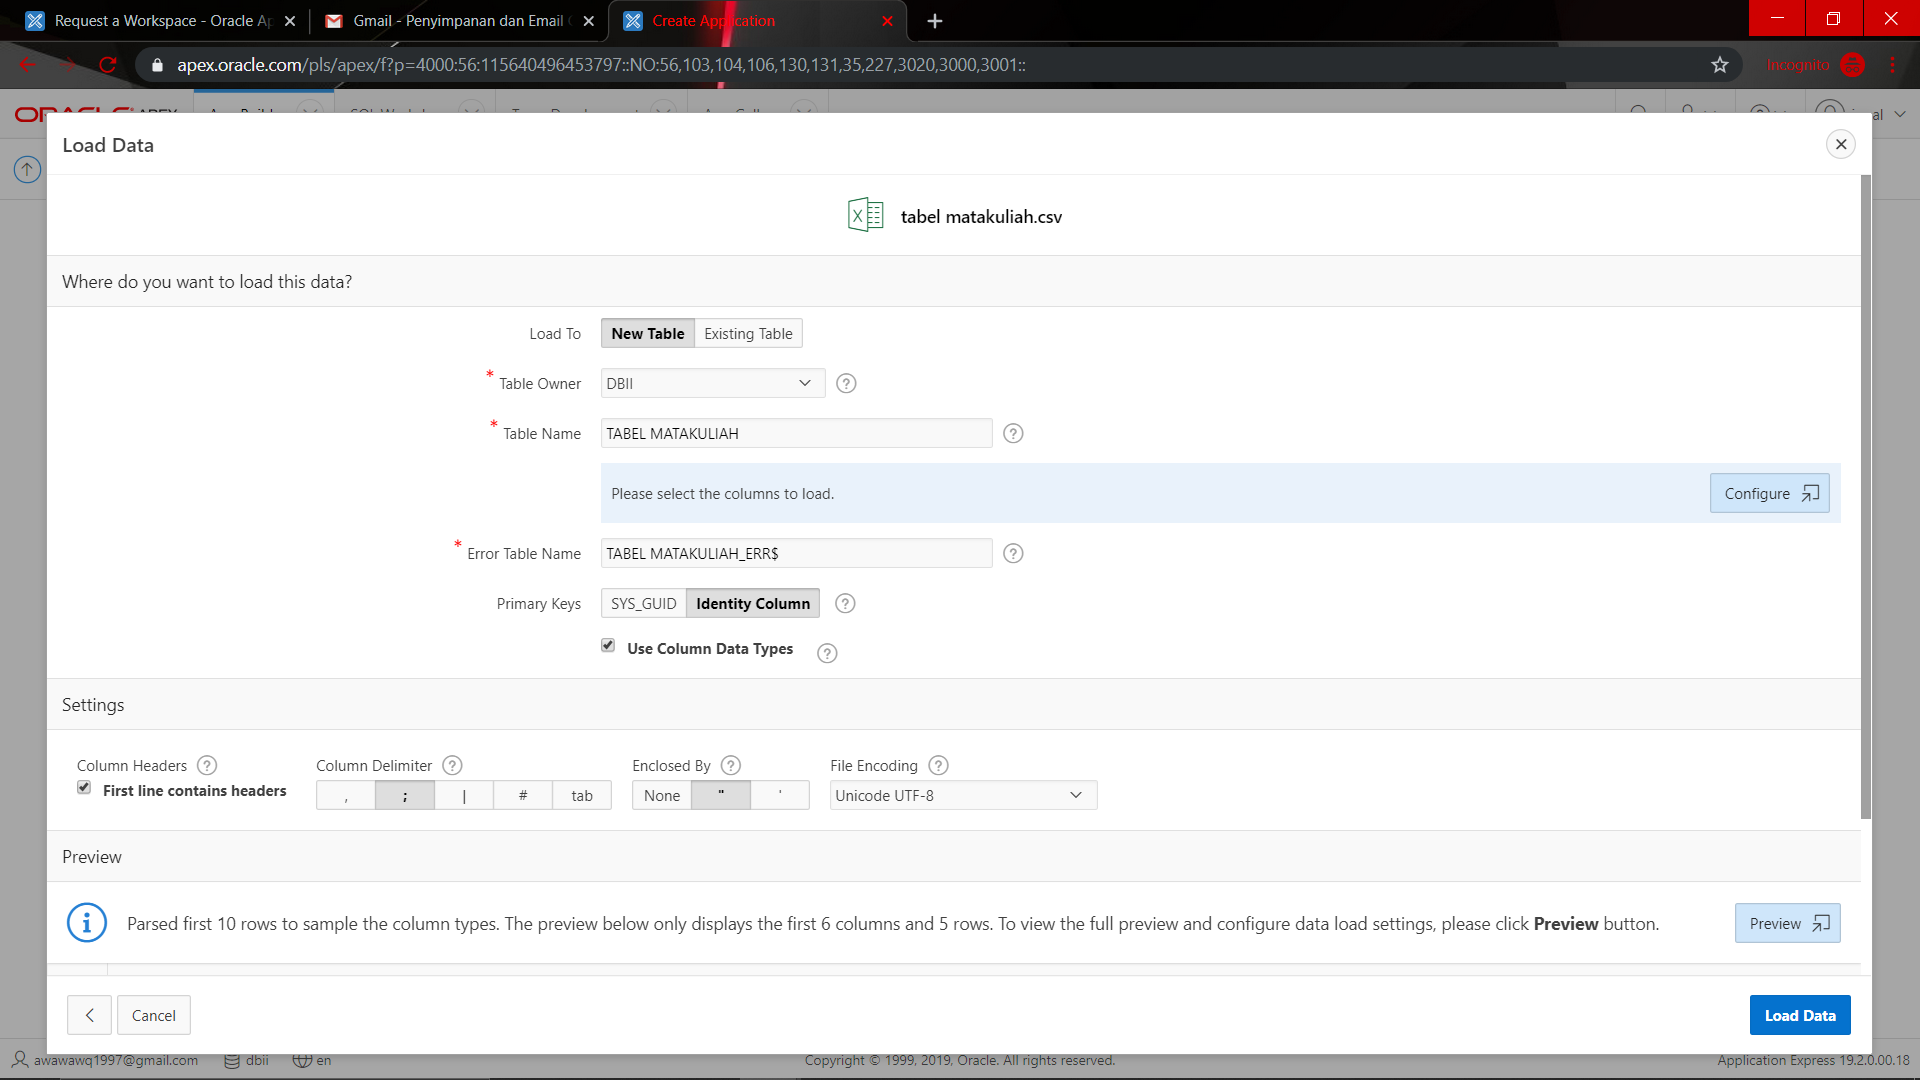
\includegraphics[scale=0.1]{figures/15}
    \caption{}
    \label{Environment1}
\end{figure}

\item untuk melihat file tabel yang sudah dimasukan klik error table dan klik configure
\begin{figure}[H]
    \centering
    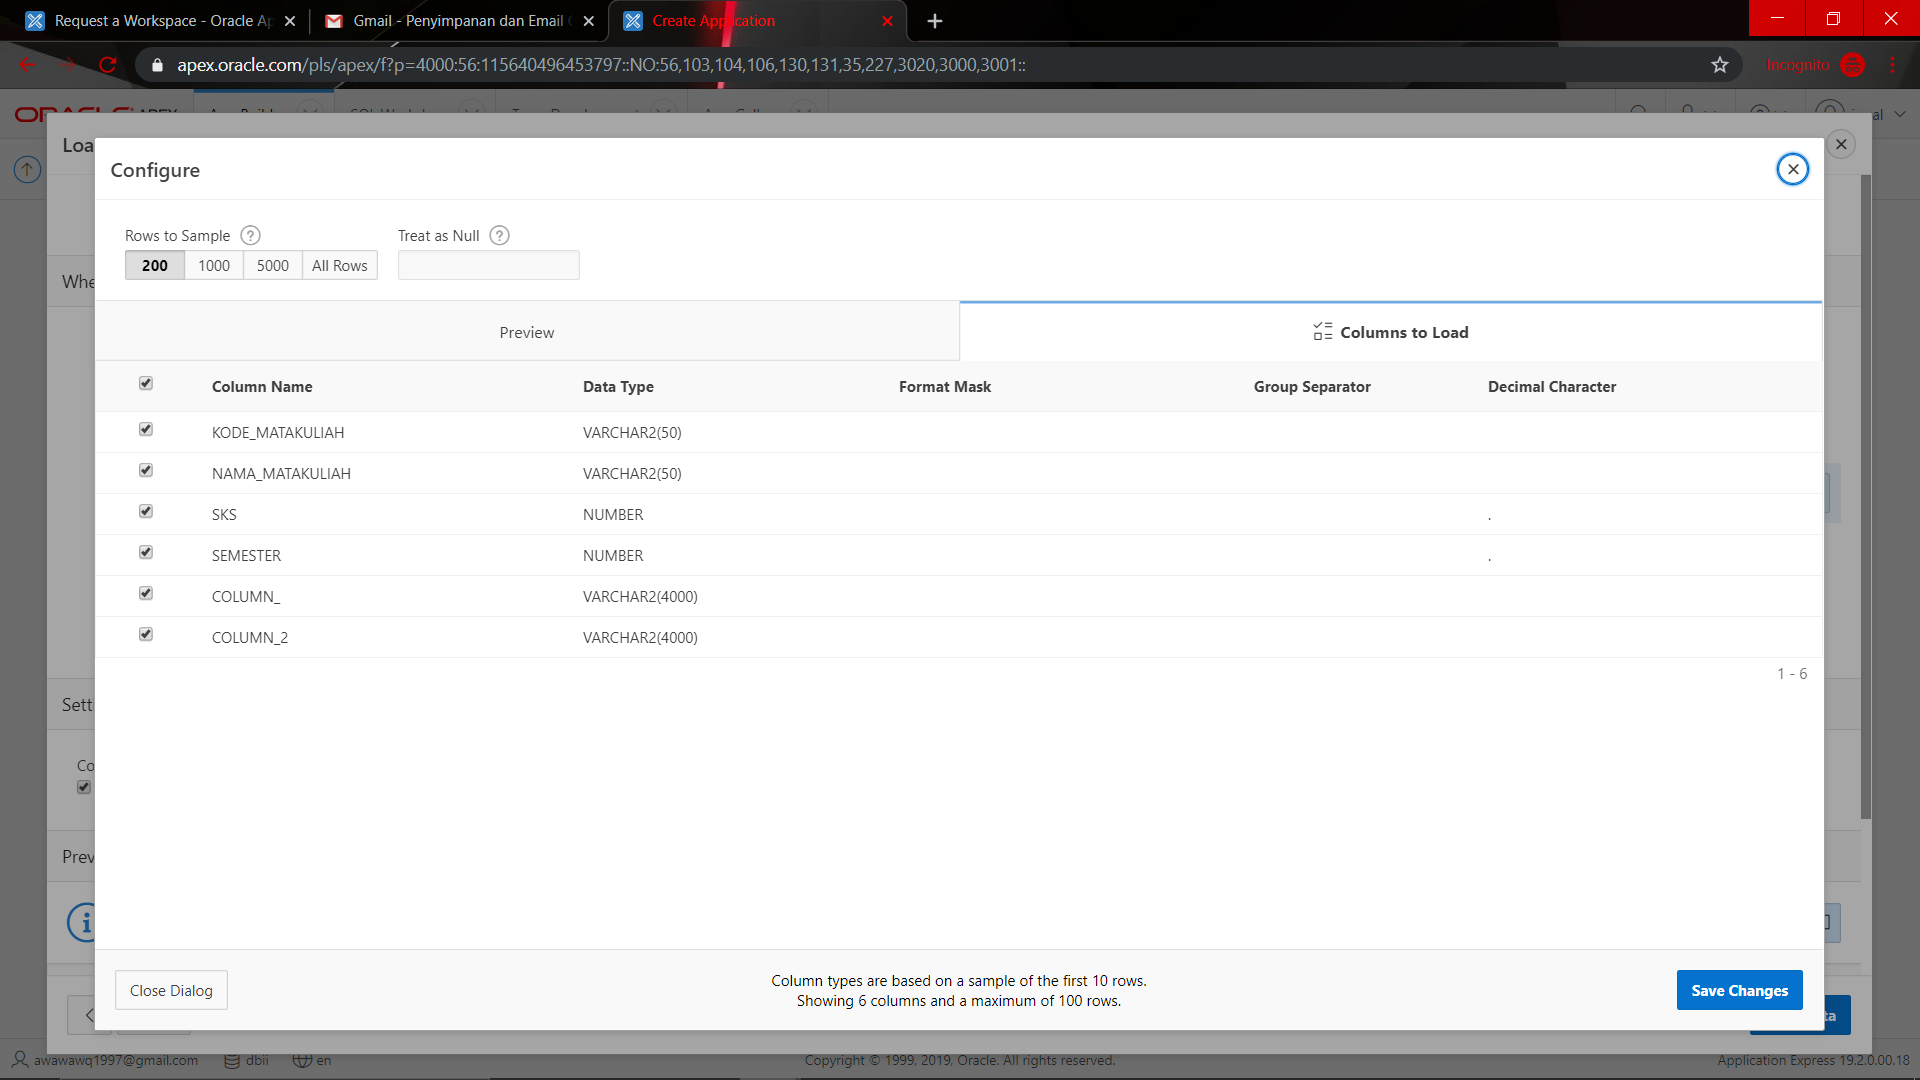
\includegraphics[scale=0.1]{figures/16}
    \caption{}
    \label{Environment2}
\end{figure}

\item selanjutnya masukan kembali file yang ingin dimasukan 
\begin{figure}[H]
    \centering
    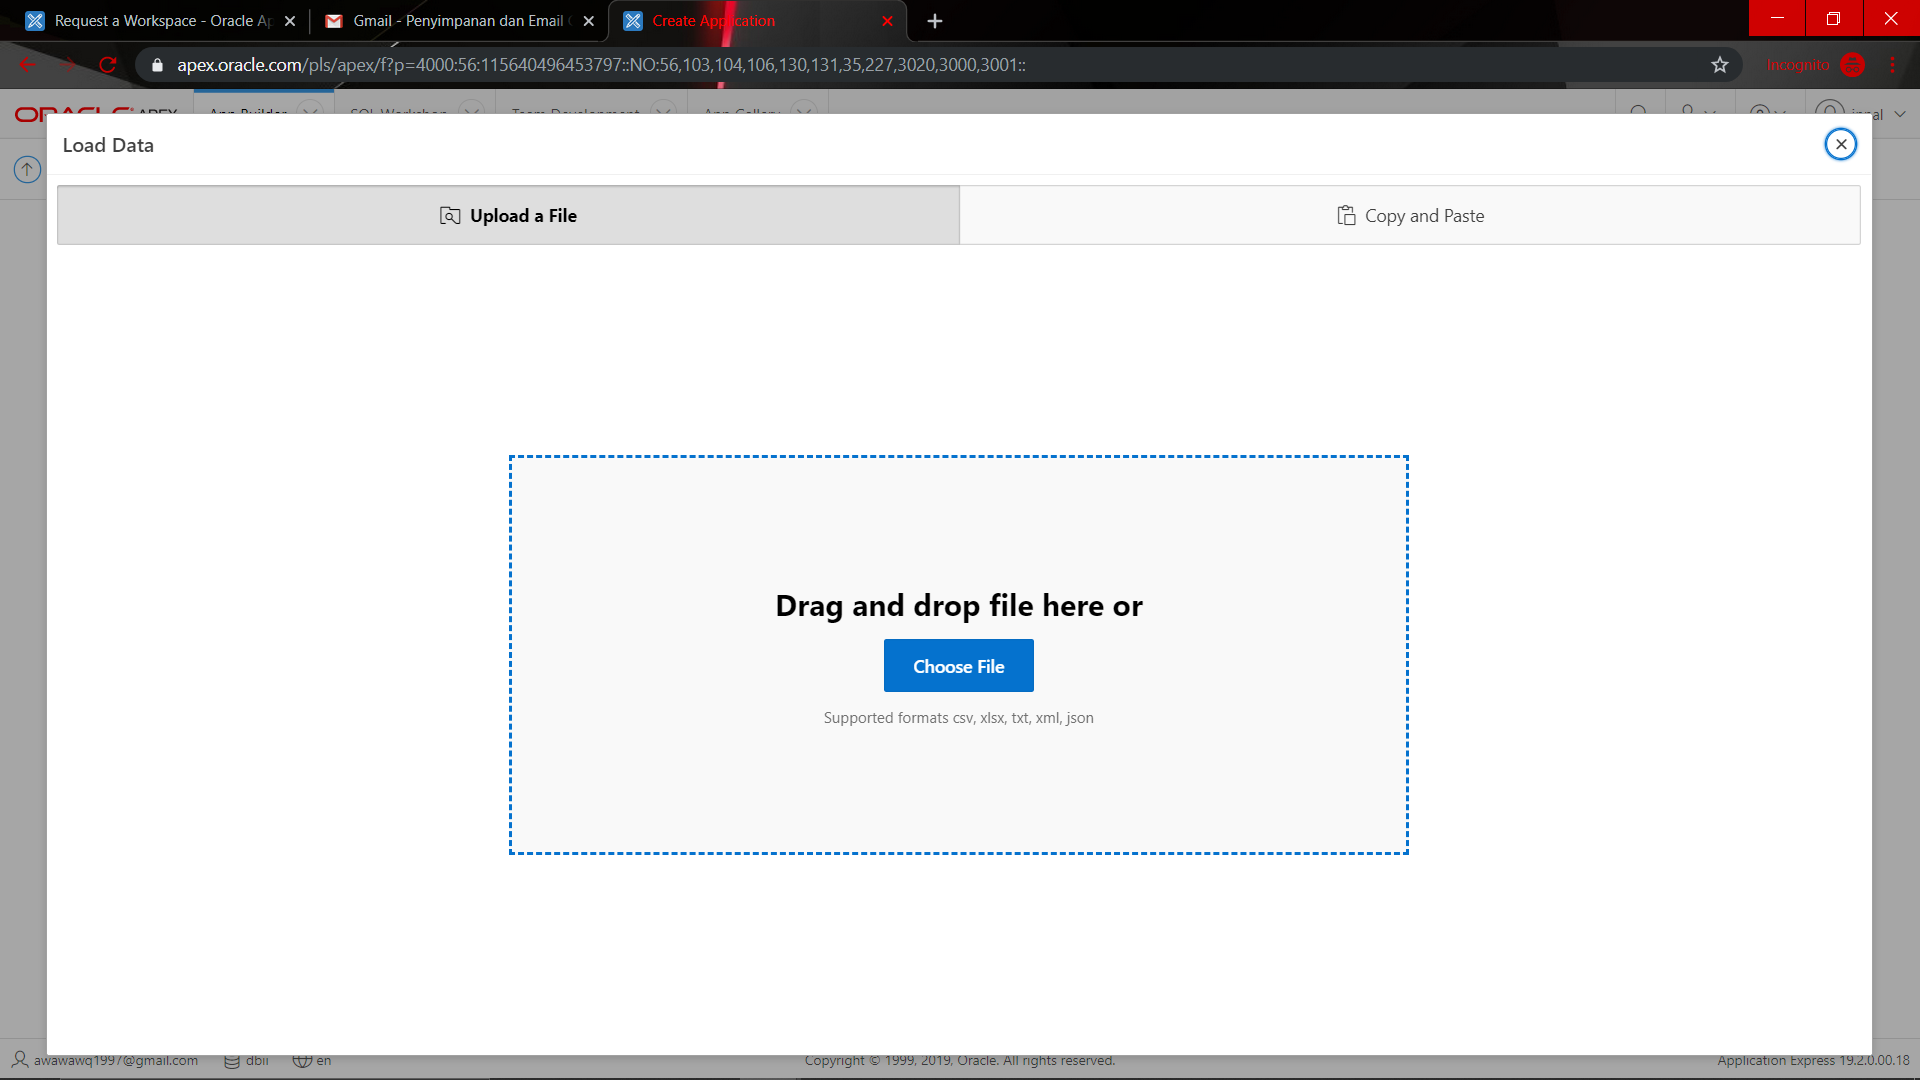
\includegraphics[scale=0.1]{figures/17}
    \caption{}
    \label{Environment3}
\end{figure}

\item berikan nama untuk file tersebut
\begin{figure}[H]
    \centering
    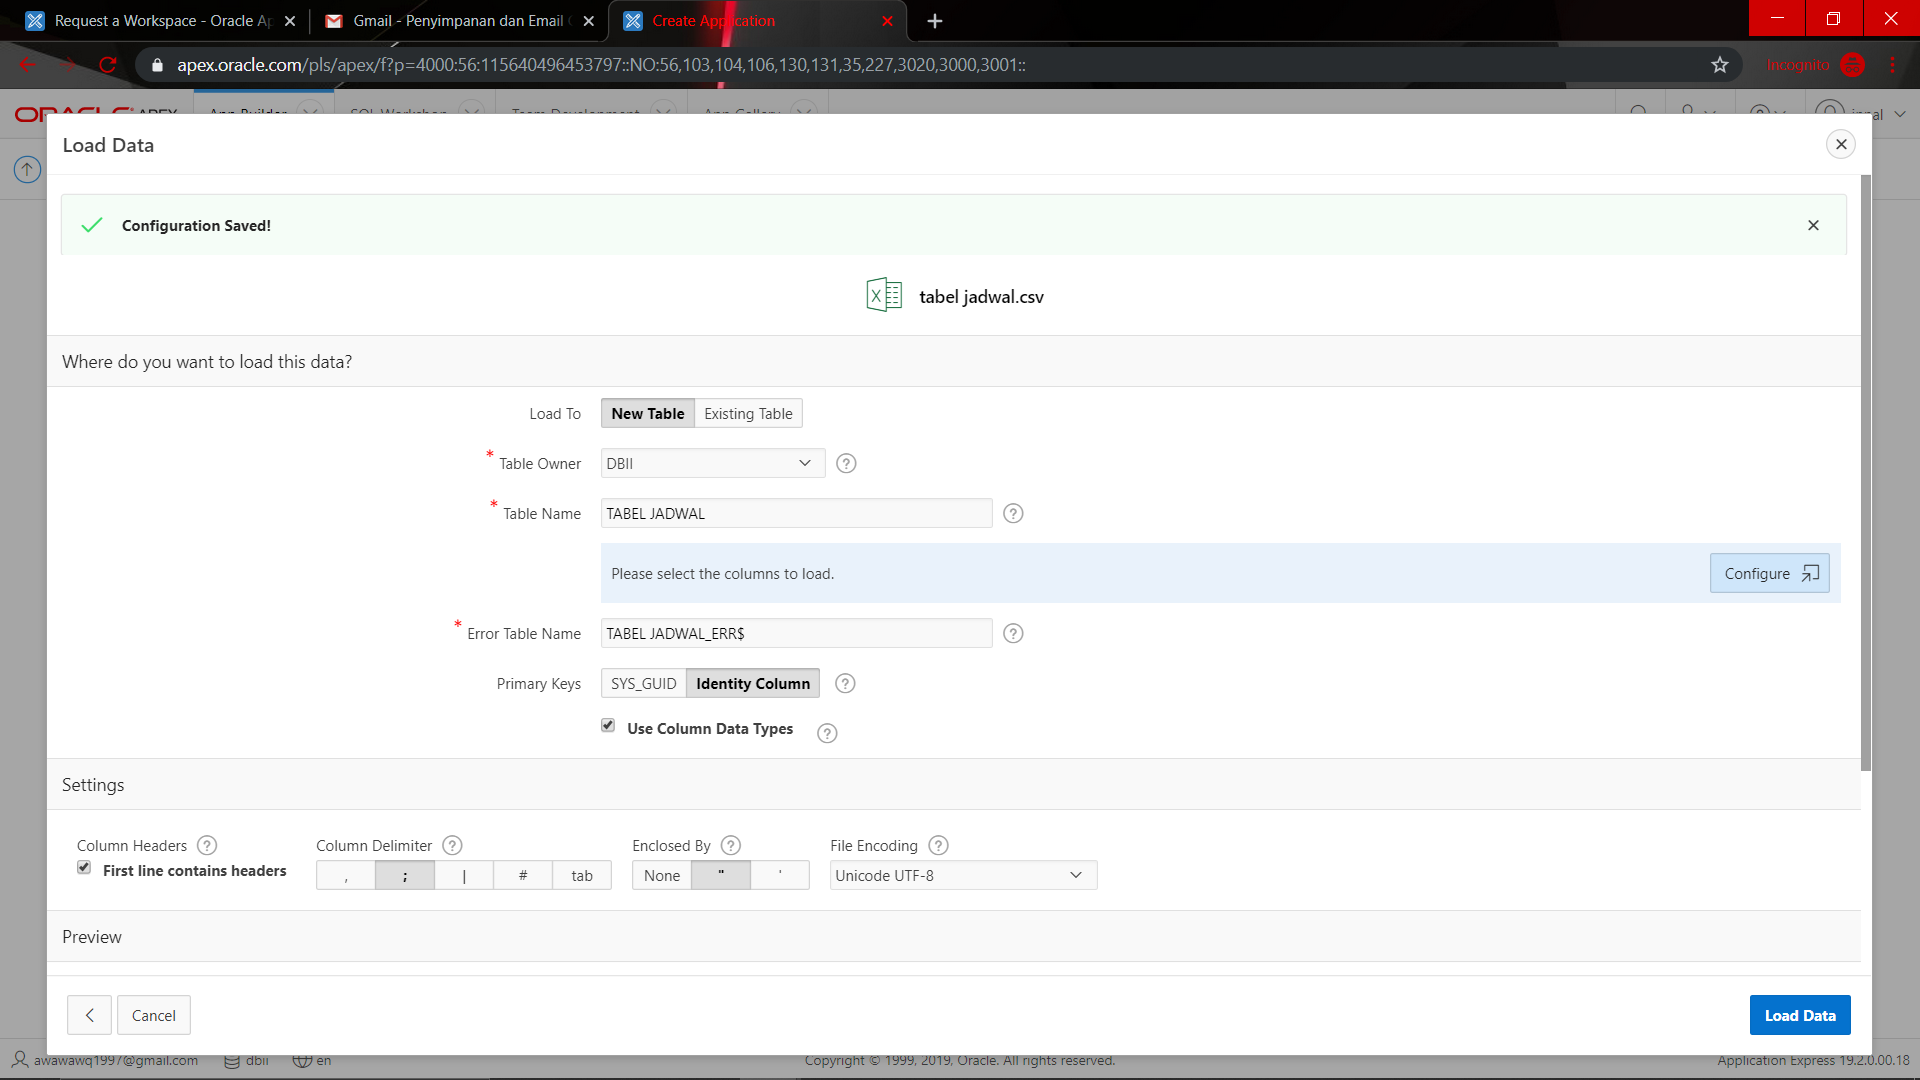
\includegraphics[scale=0.1]{figures/18}
    \caption{}
    \label{Environment4}
\end{figure}

\item lalu klik create application
\begin{figure}[H]
    \centering
    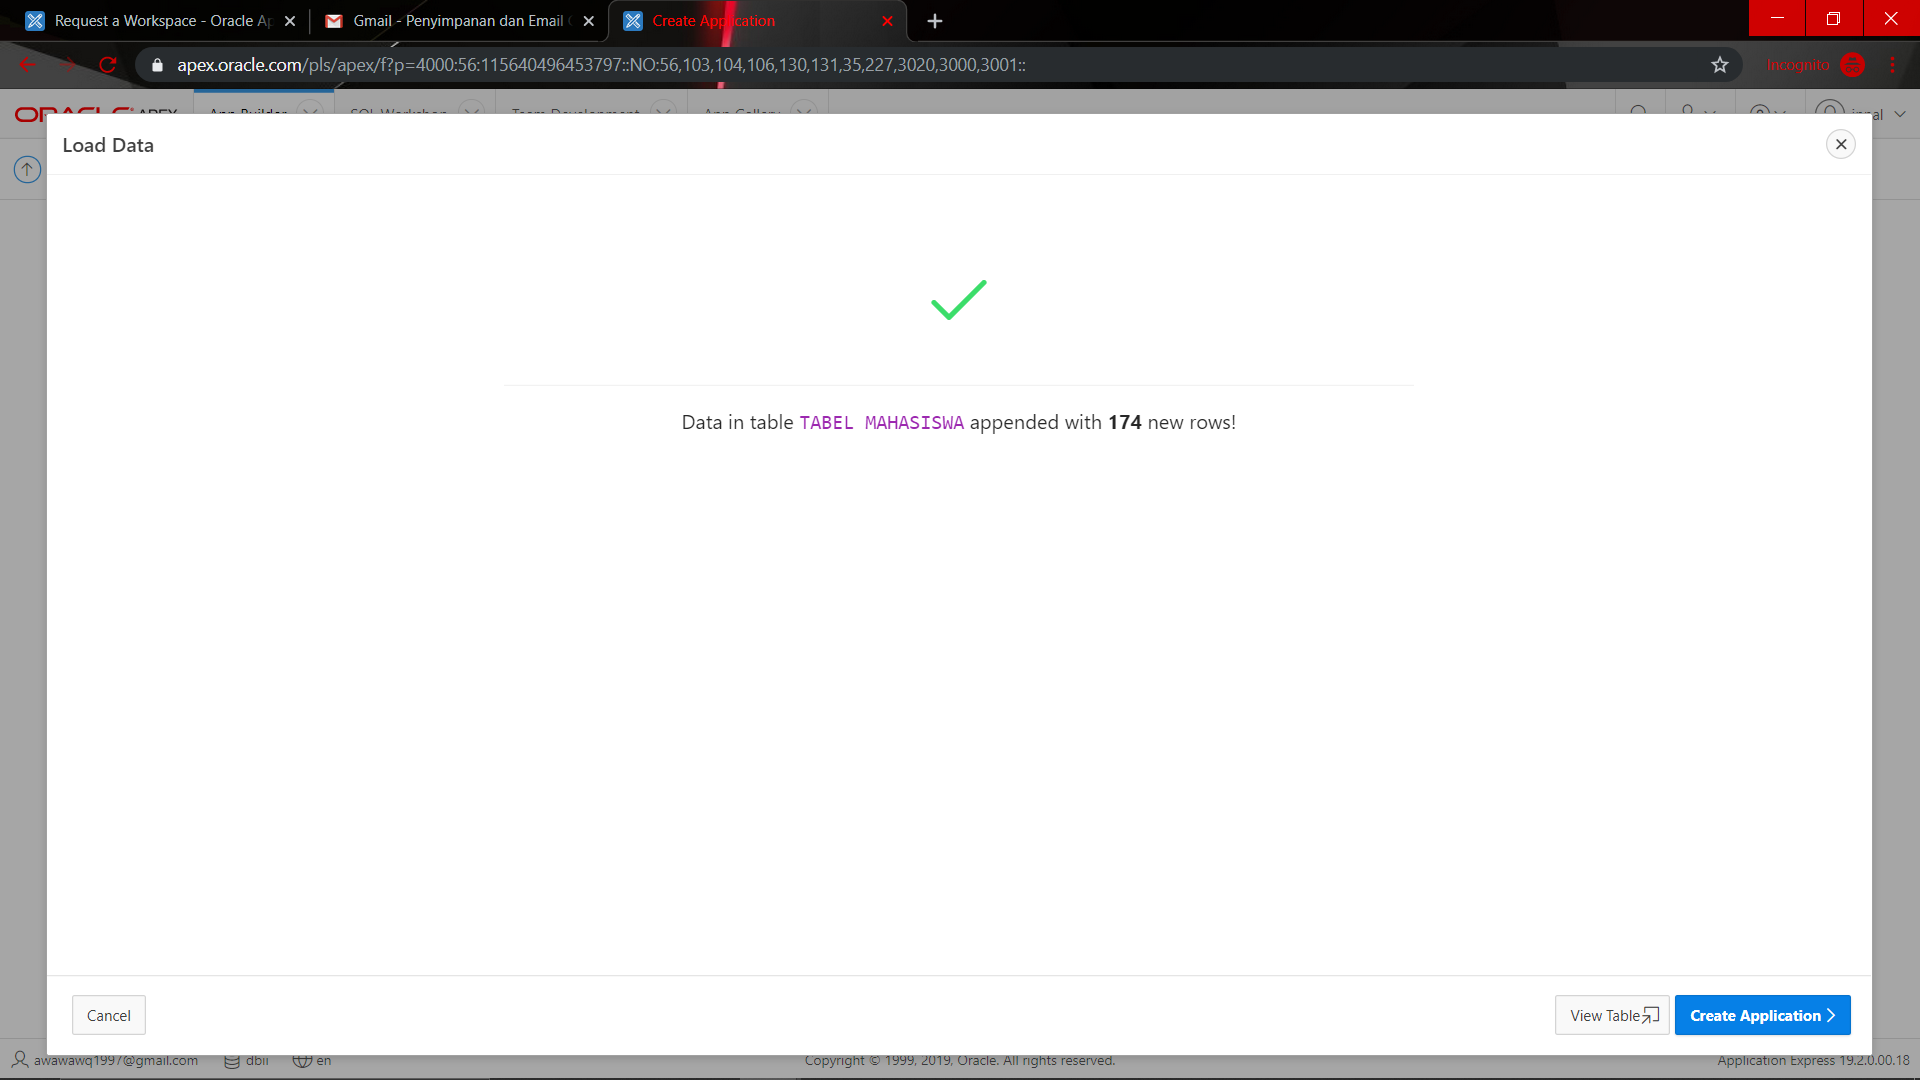
\includegraphics[scale=0.1]{figures/19}
    \caption{}
    \label{Environment5}
\end{figure}

\item setelah itu klik add page 
\begin{figure}[H]
    \centering
    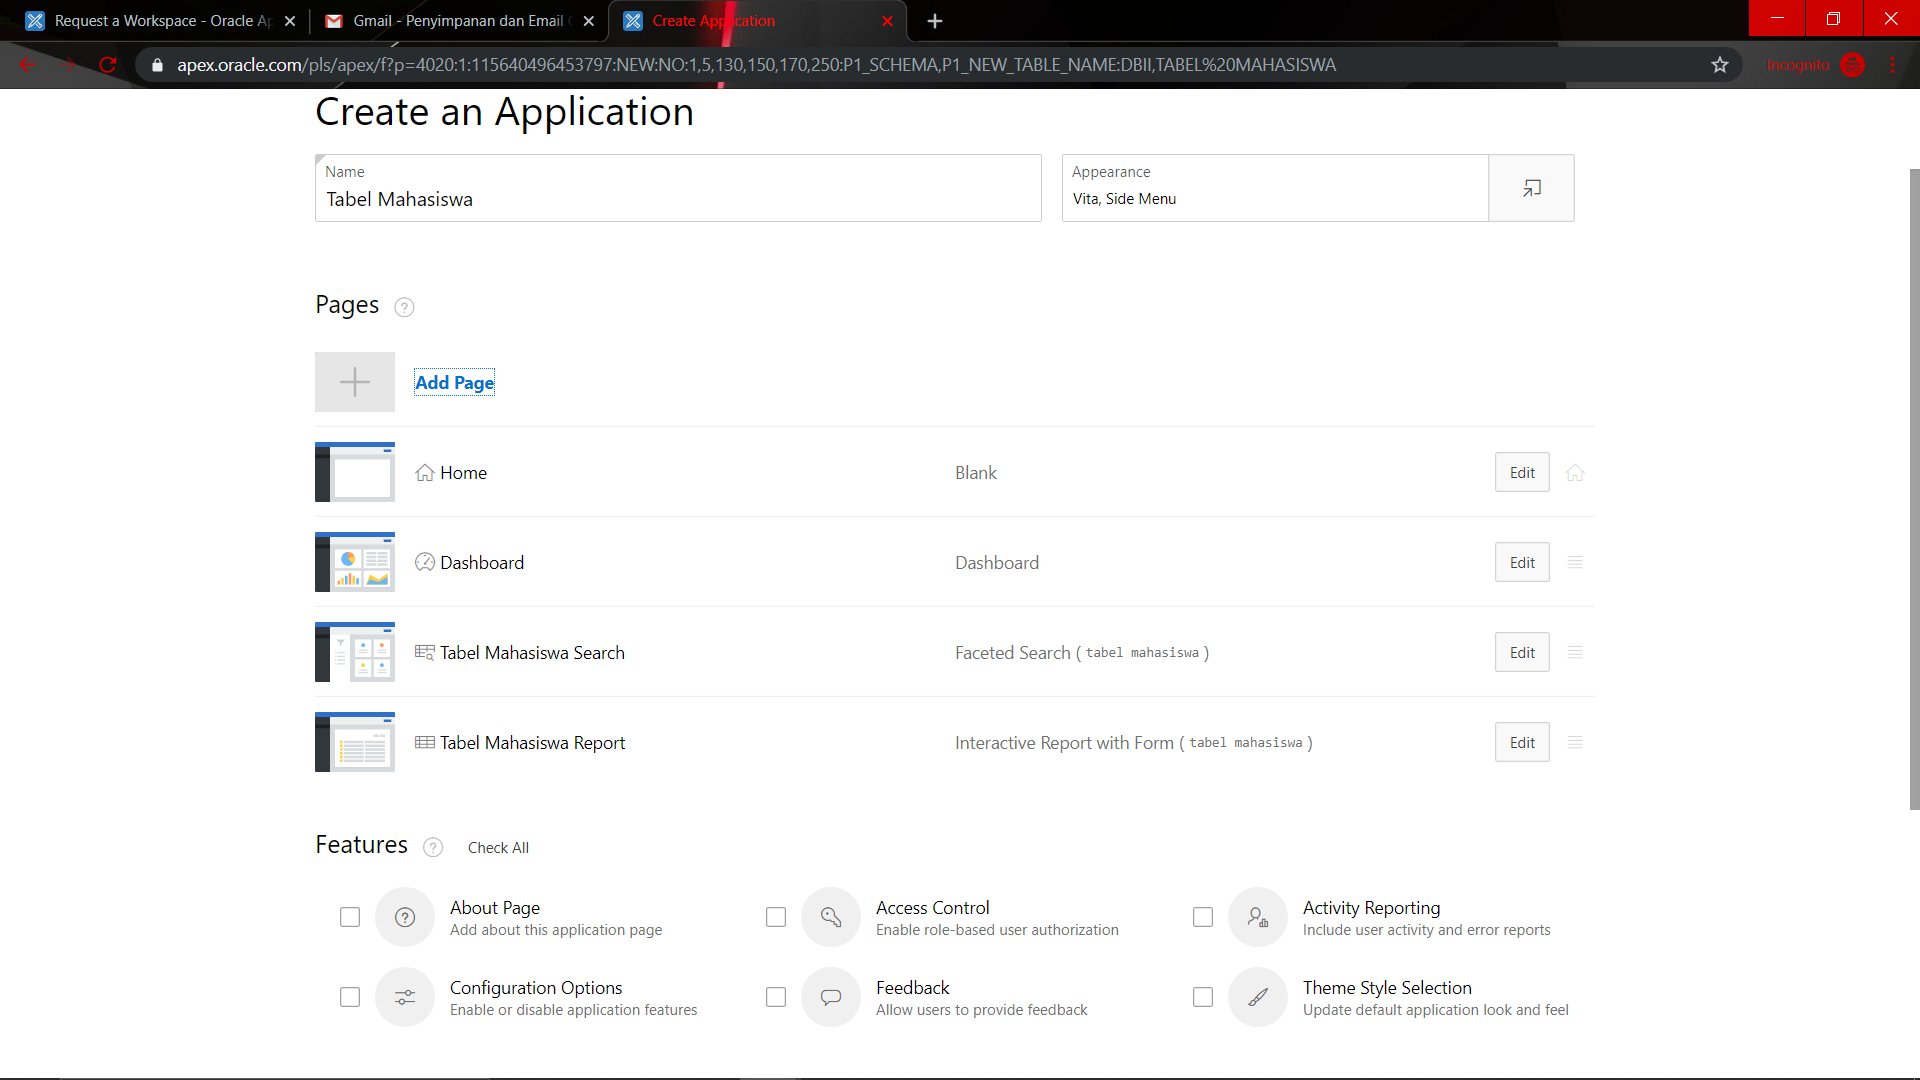
\includegraphics[scale=0.1]{figures/20}
    \caption{}
    \label{CLI}
\end{figure}


\item klik interactive report
\begin{figure}[H]
    \centering
    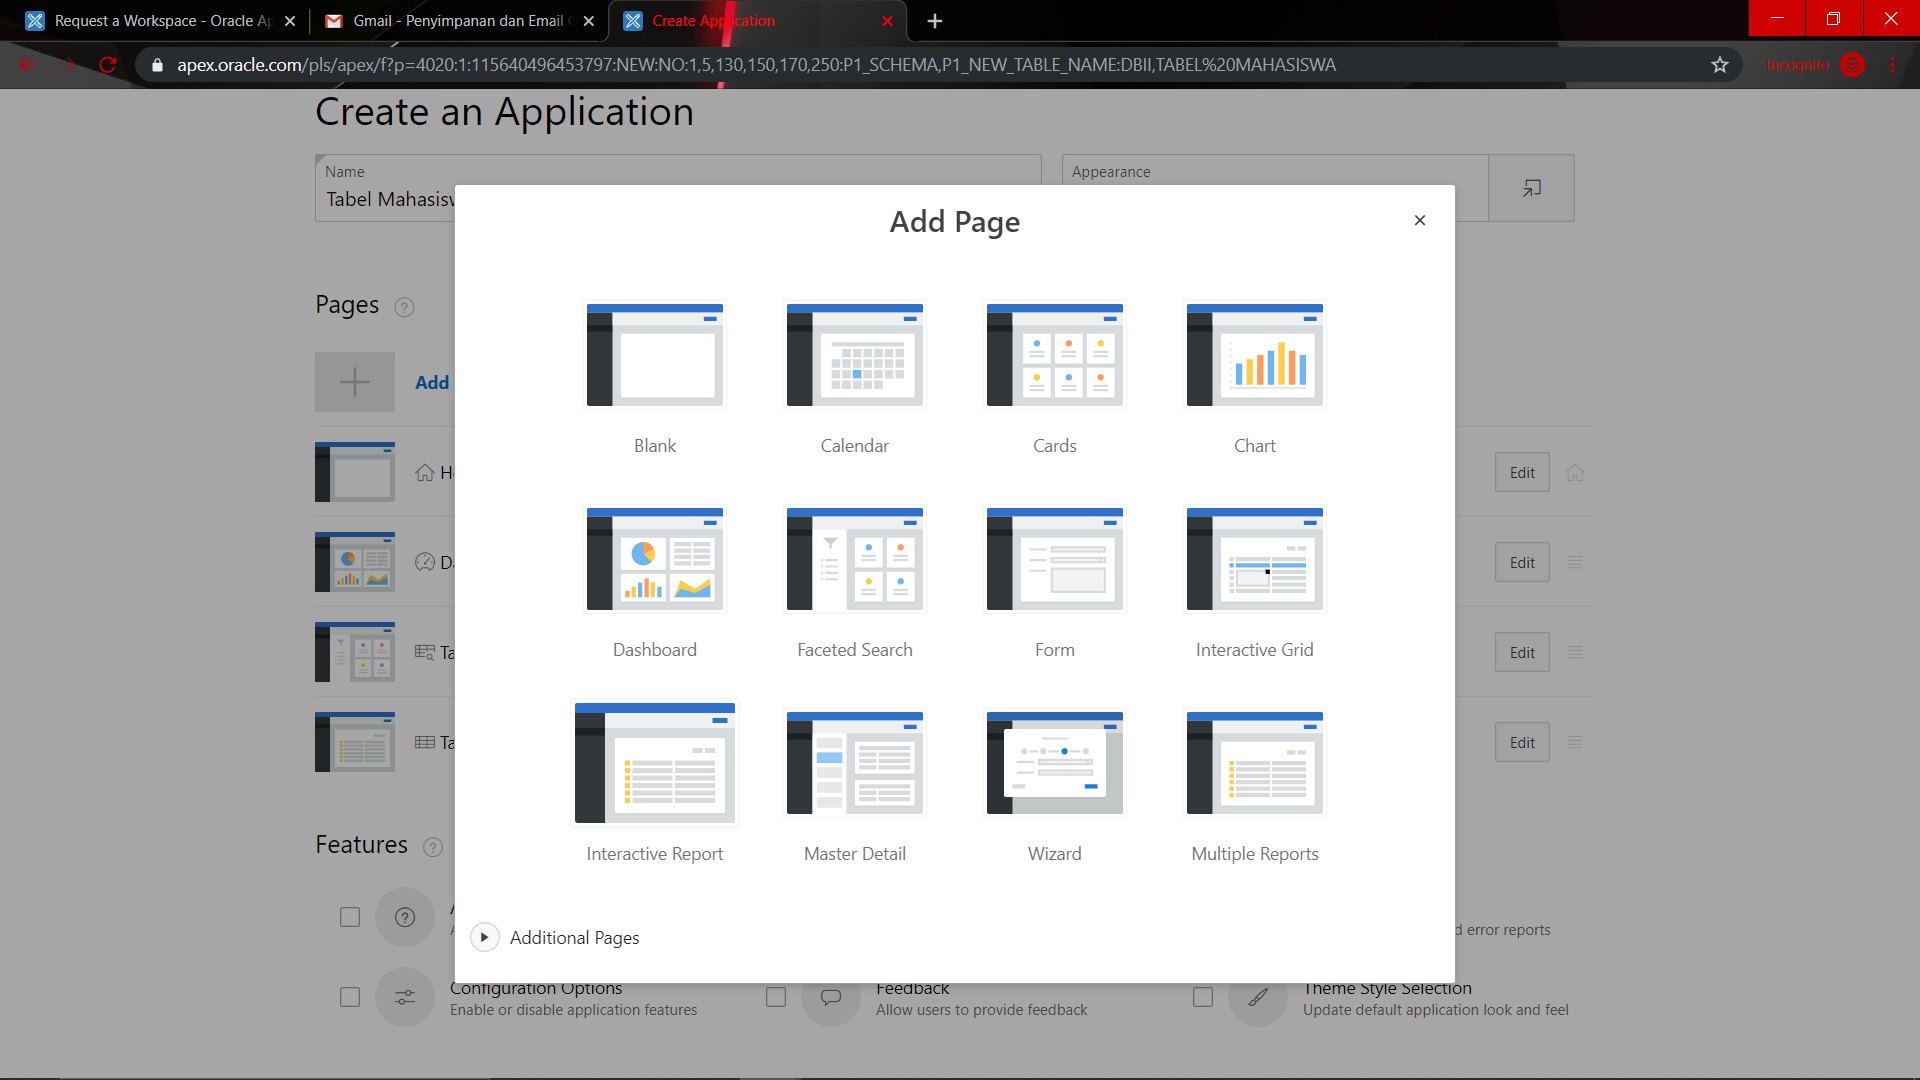
\includegraphics[scale=0.1]{figures/21}
    \caption{}
    \label{Anaconda Navigator}
\end{figure}

\item berikan nama page tersebut klik table or view dan klik table yang ingin di masukan ke page itu.
\begin{figure}[H]
    \centering
    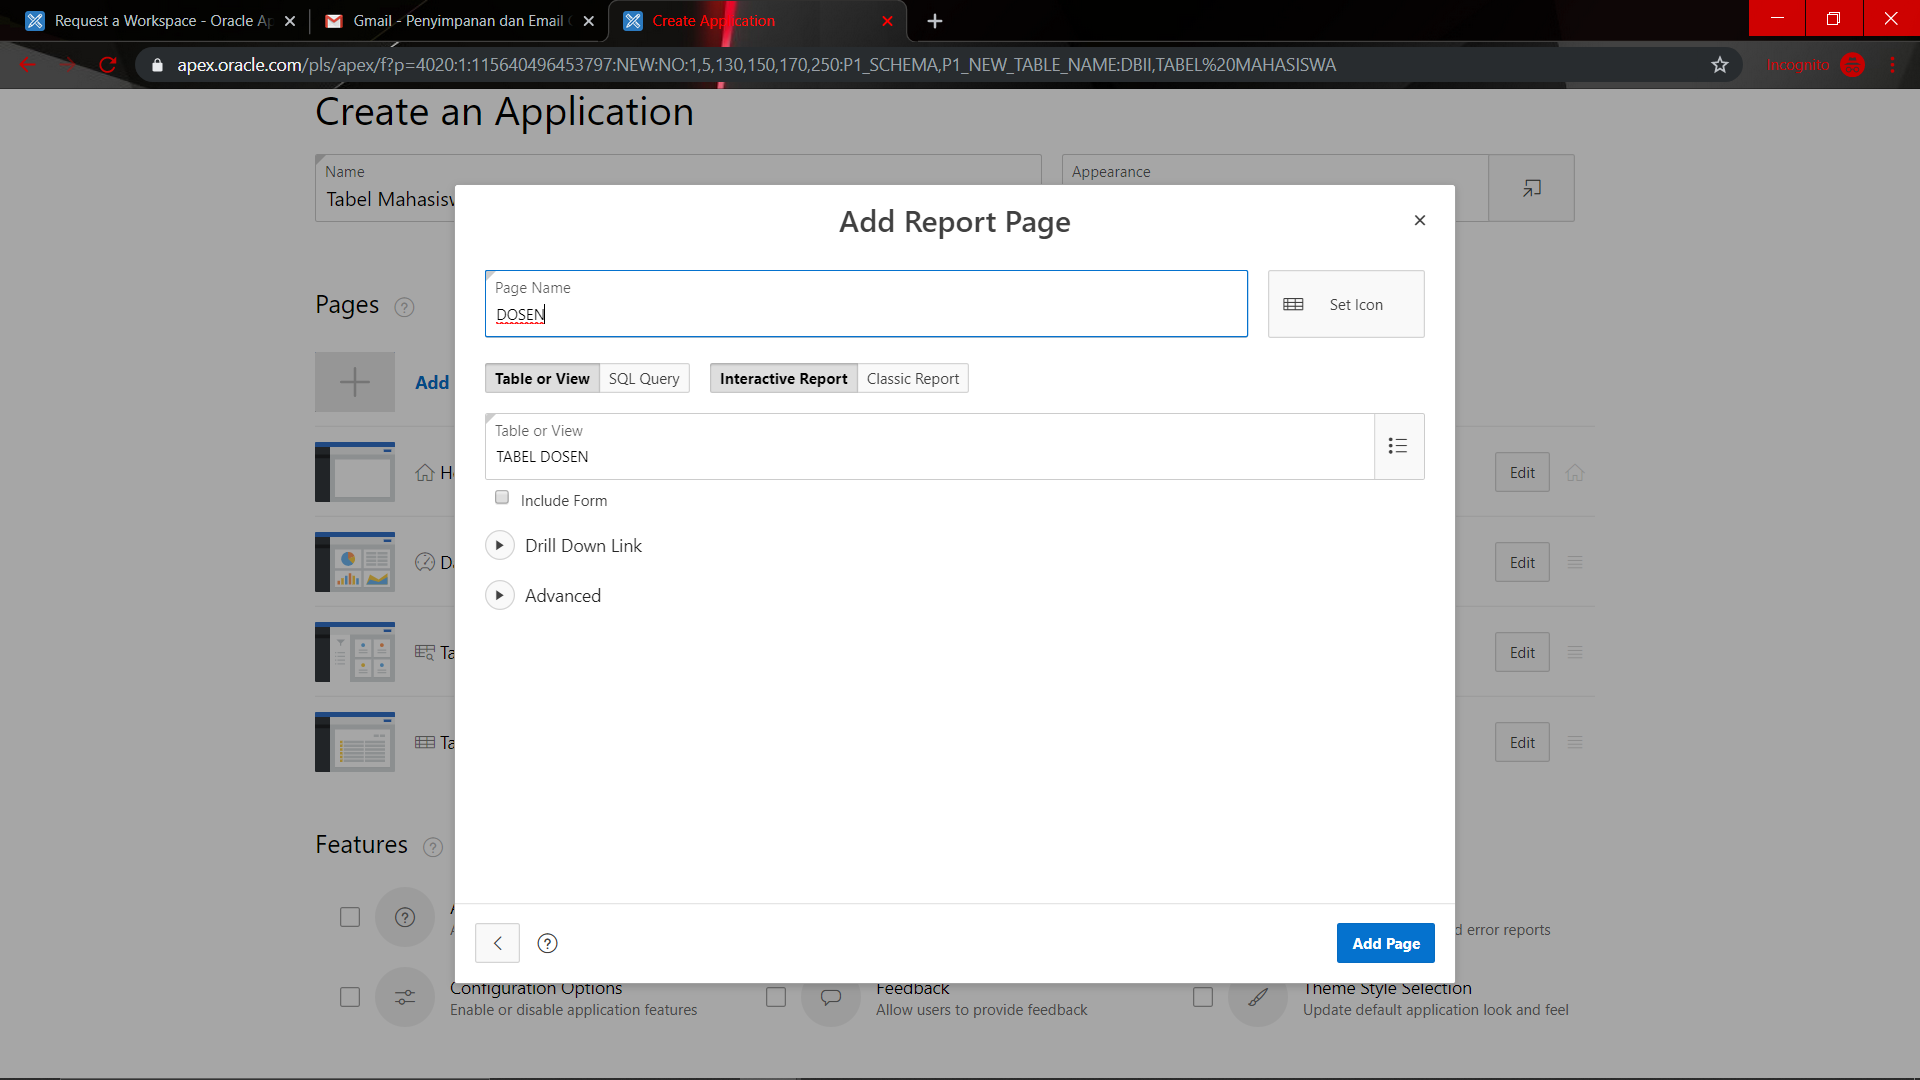
\includegraphics[scale=0.1]{figures/22}
    \caption{}
    \label{Print Hello World}
\end{figure}

\item lakukan hal yang sama seperti sebelumnya tetapi pilih table yang lain yang ingin di masukan
\begin{figure}[H]
    \centering
    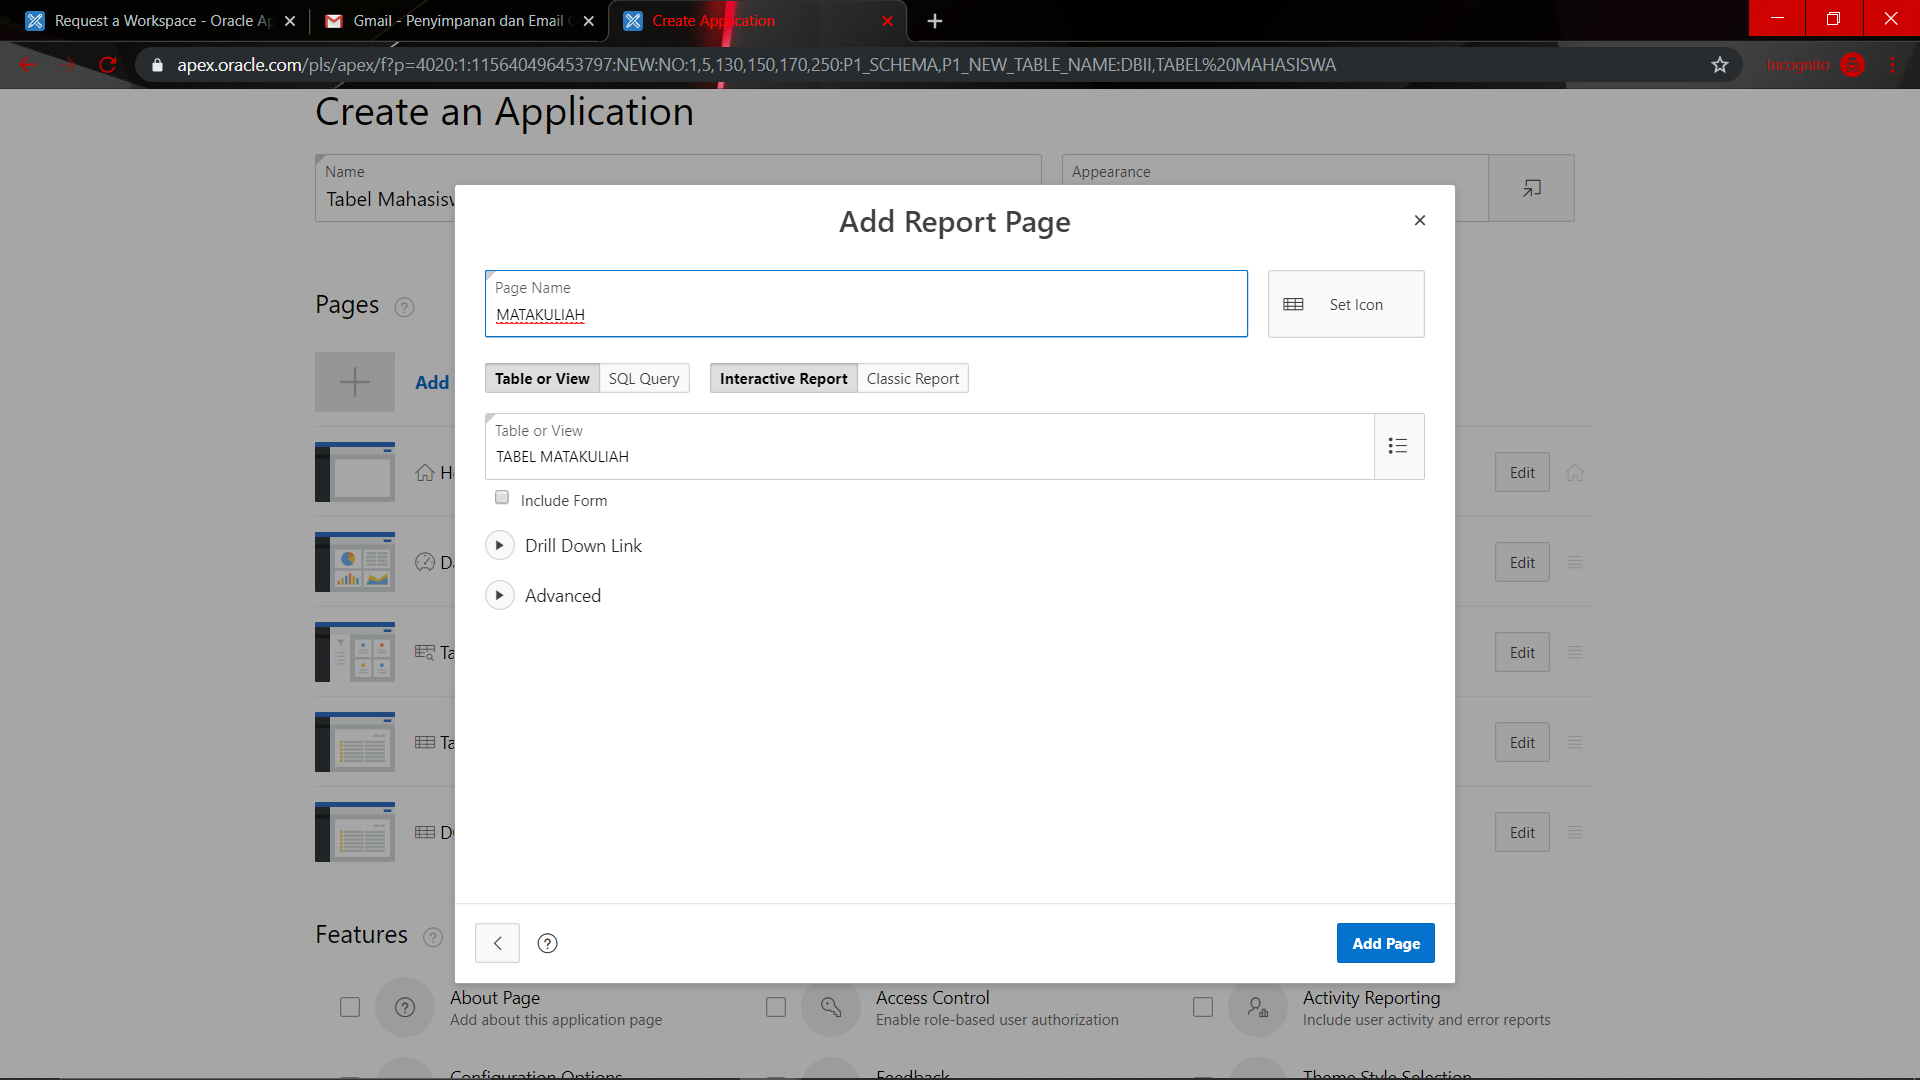
\includegraphics[scale=0.1]{figures/23}
    \caption{}
    \label{Hello World}
\end{figure}

\item lakukan hal yang sama seperti sebelumnya tetapi pilih table yang lain yang ingin di masukan
\begin{figure}[H]
    \centering
    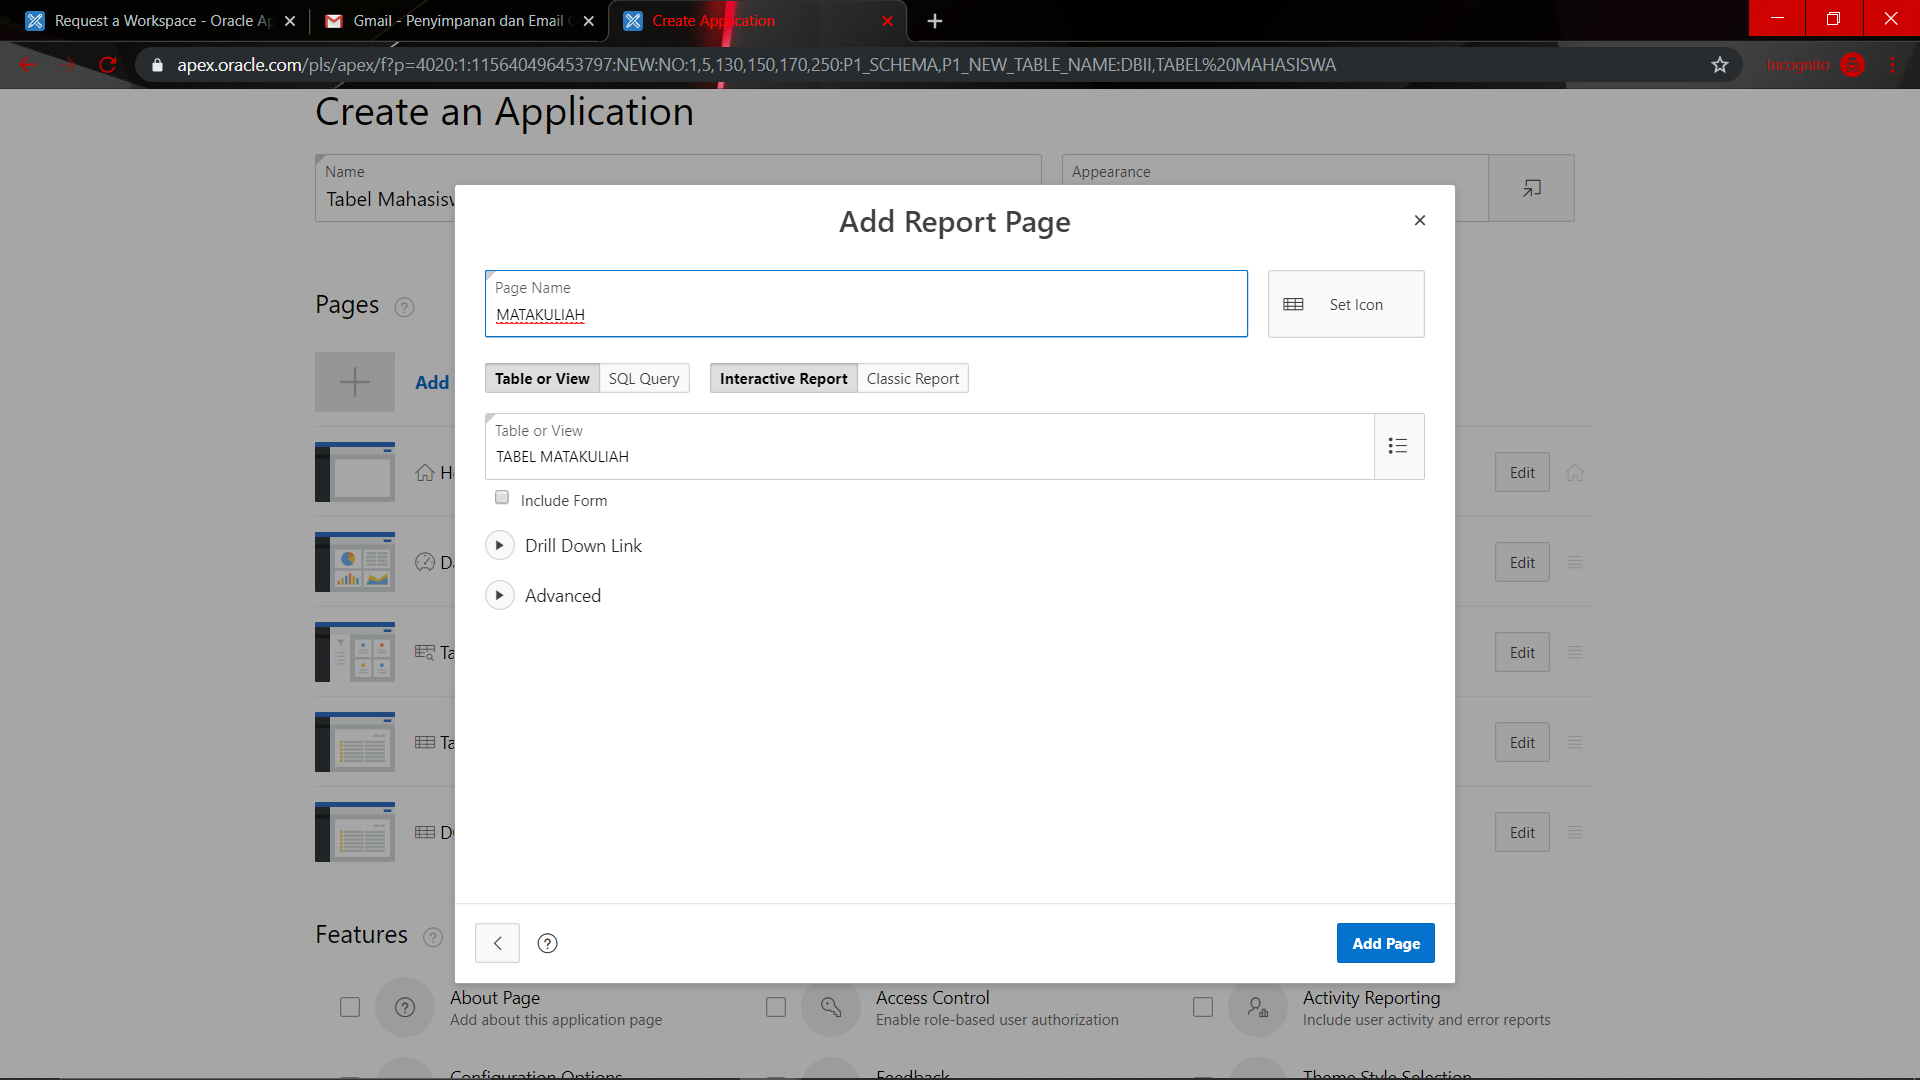
\includegraphics[scale=0.1]{figures/23}
    \caption{}
    \label{Automatic1}
\end{figure}

\item lakukan hal yang sama seperti sebelumnya tetapi pilih table yang lain yang ingin di masukan
\begin{figure}[H]
    \centering
    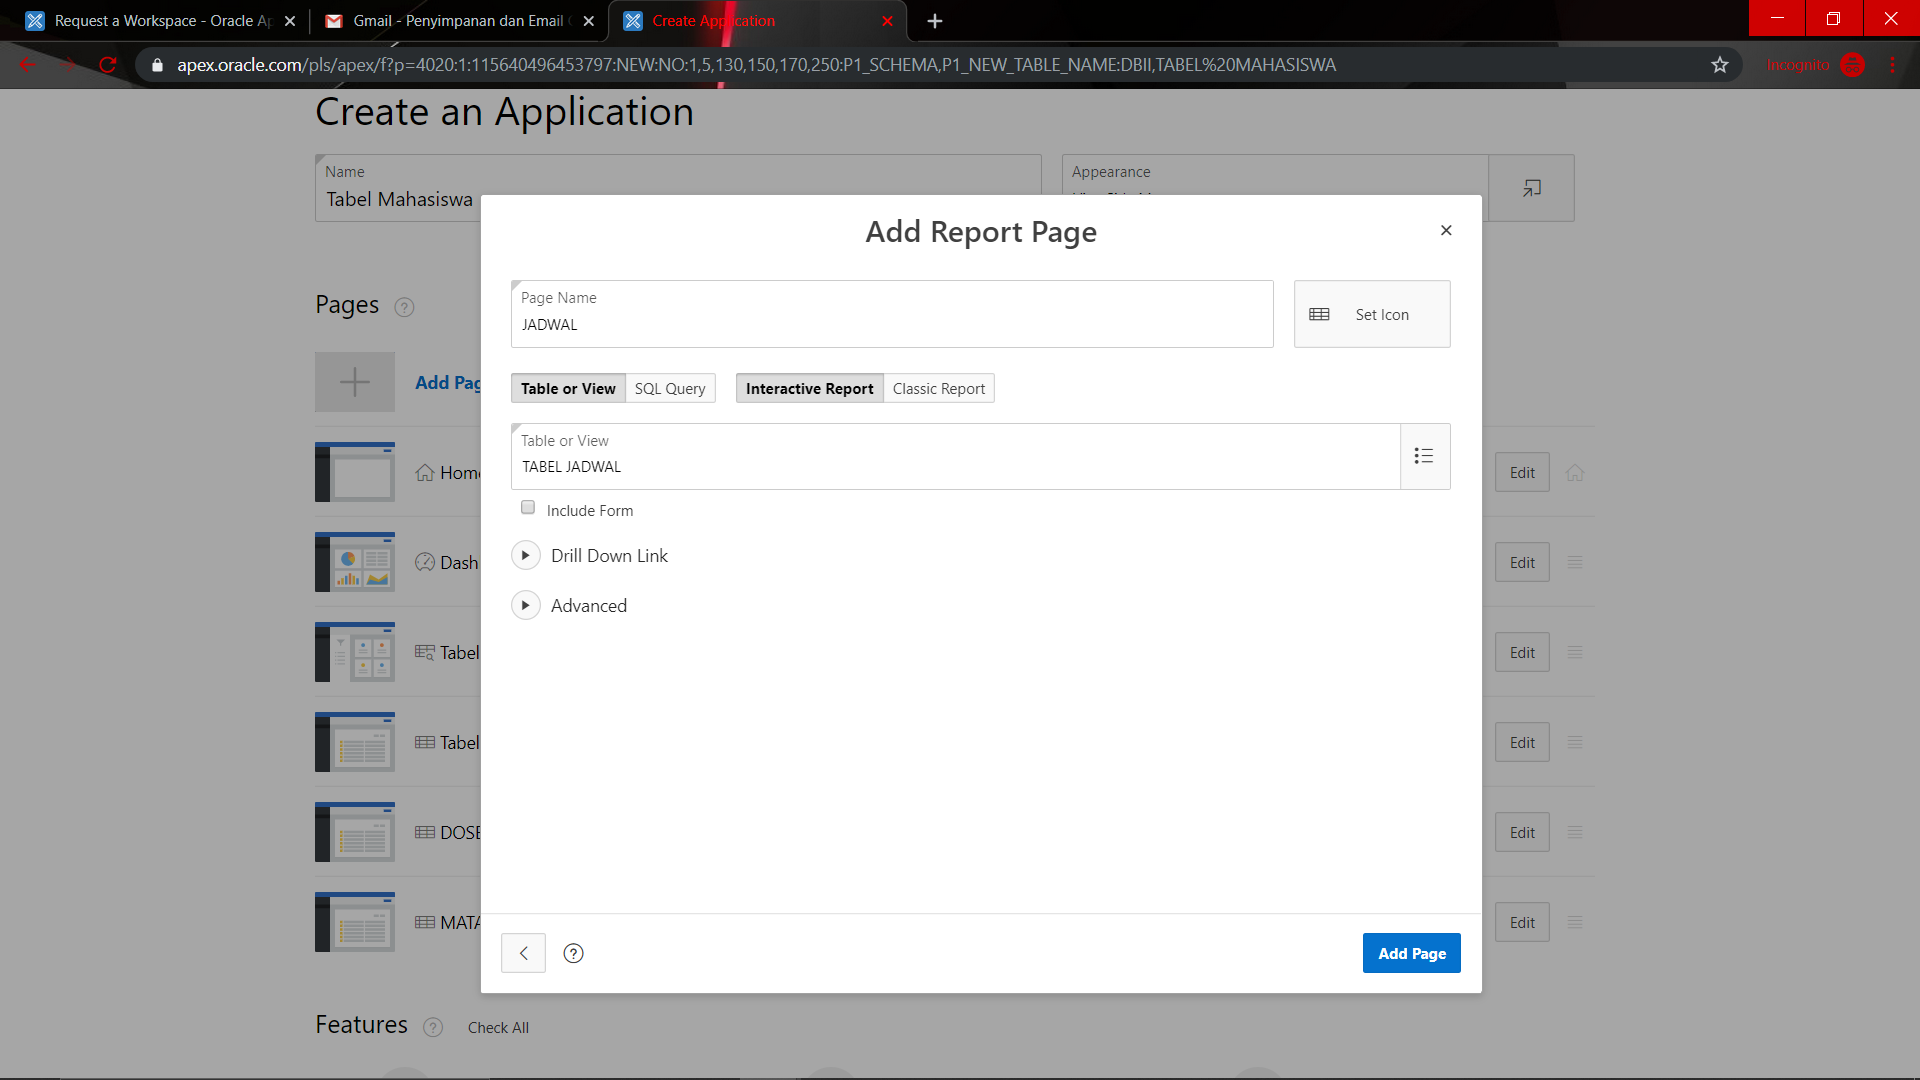
\includegraphics[scale=0.1]{figures/24}
    \caption{}
    \label{Automatic2}
\end{figure}

\item lakukan hal yang sama seperti sebelumnya tetapi pilih table yang lain yang ingin di masukan
\begin{figure}[H]
    \centering
    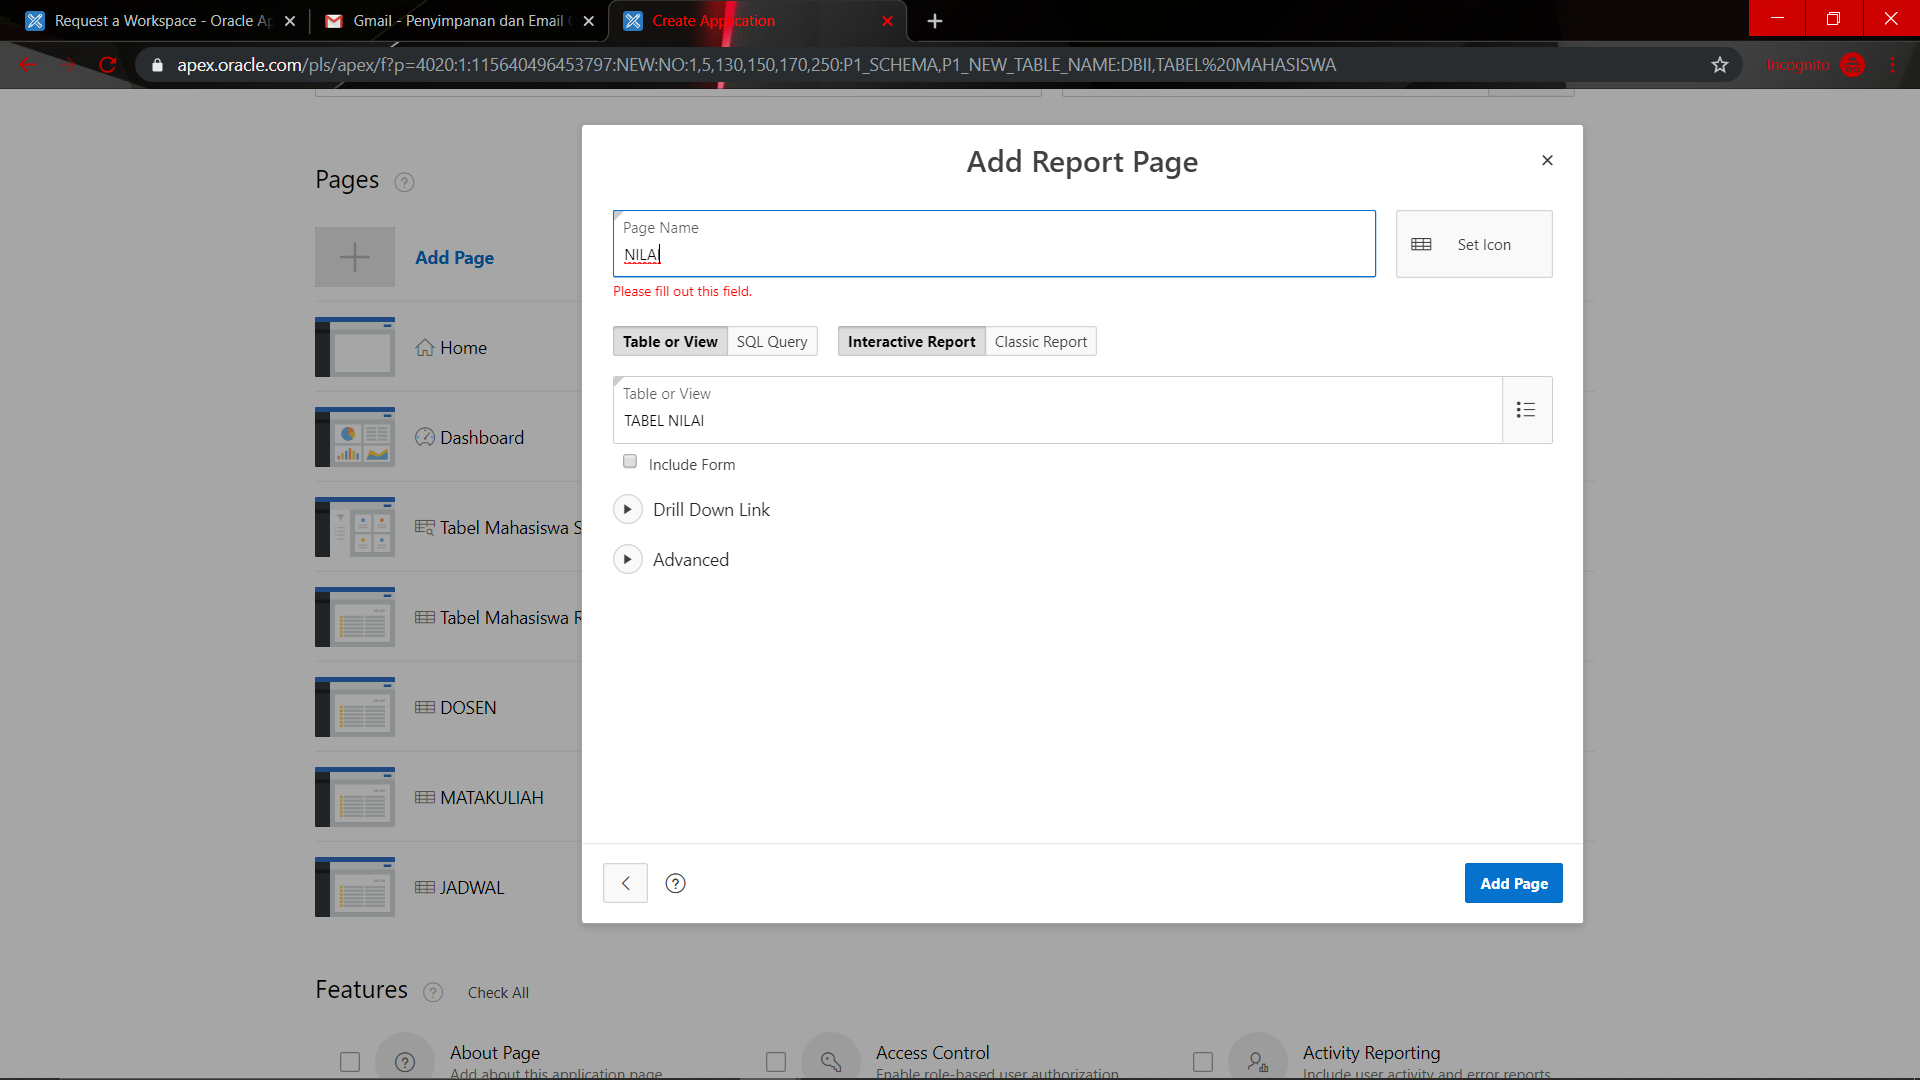
\includegraphics[scale=0.1]{figures/25}
    \caption{}
    \label{Automatic3}
\end{figure}

\item setelah memasukan semua table ke page klik create application
\begin{figure}[H]
    \centering
    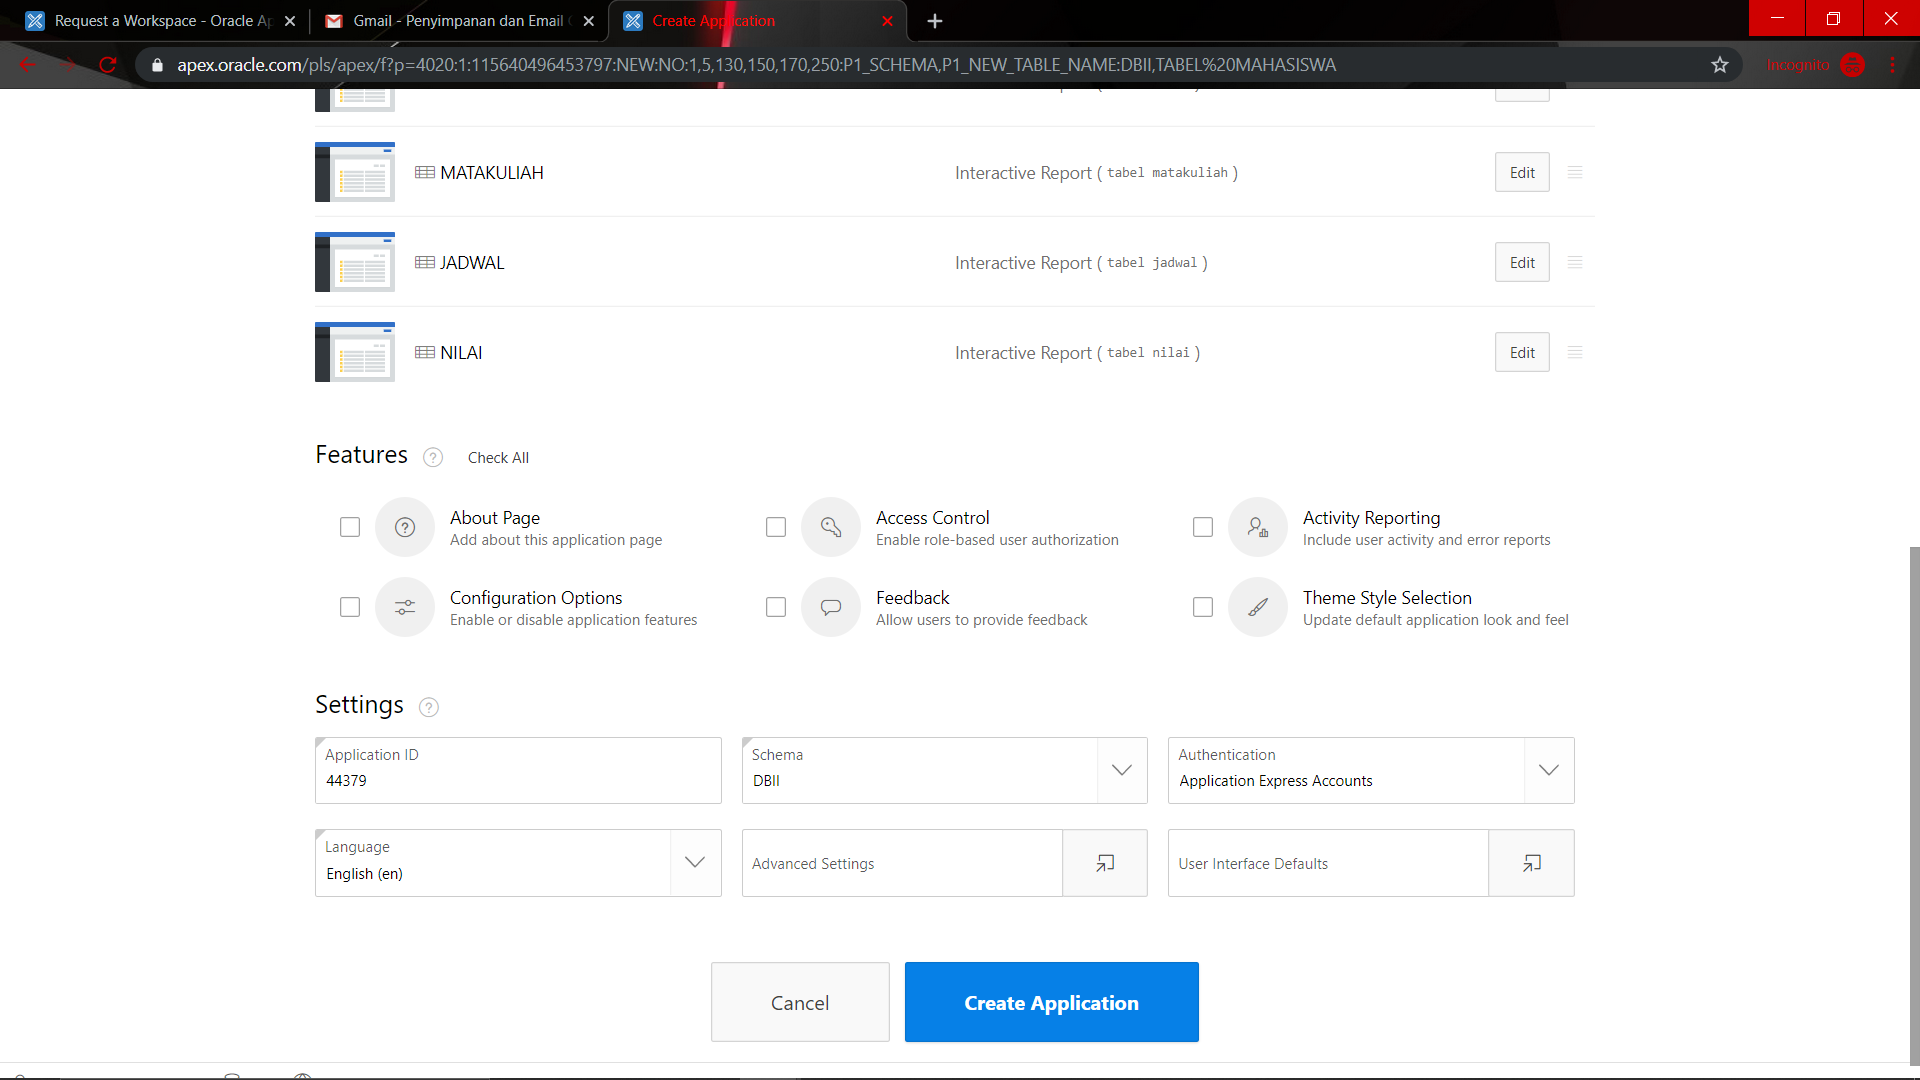
\includegraphics[scale=0.1]{figures/26}
    \caption{}
    \label{Automatic4}
\end{figure}

\item masukan username dan password
\begin{figure}[H]
    \centering
    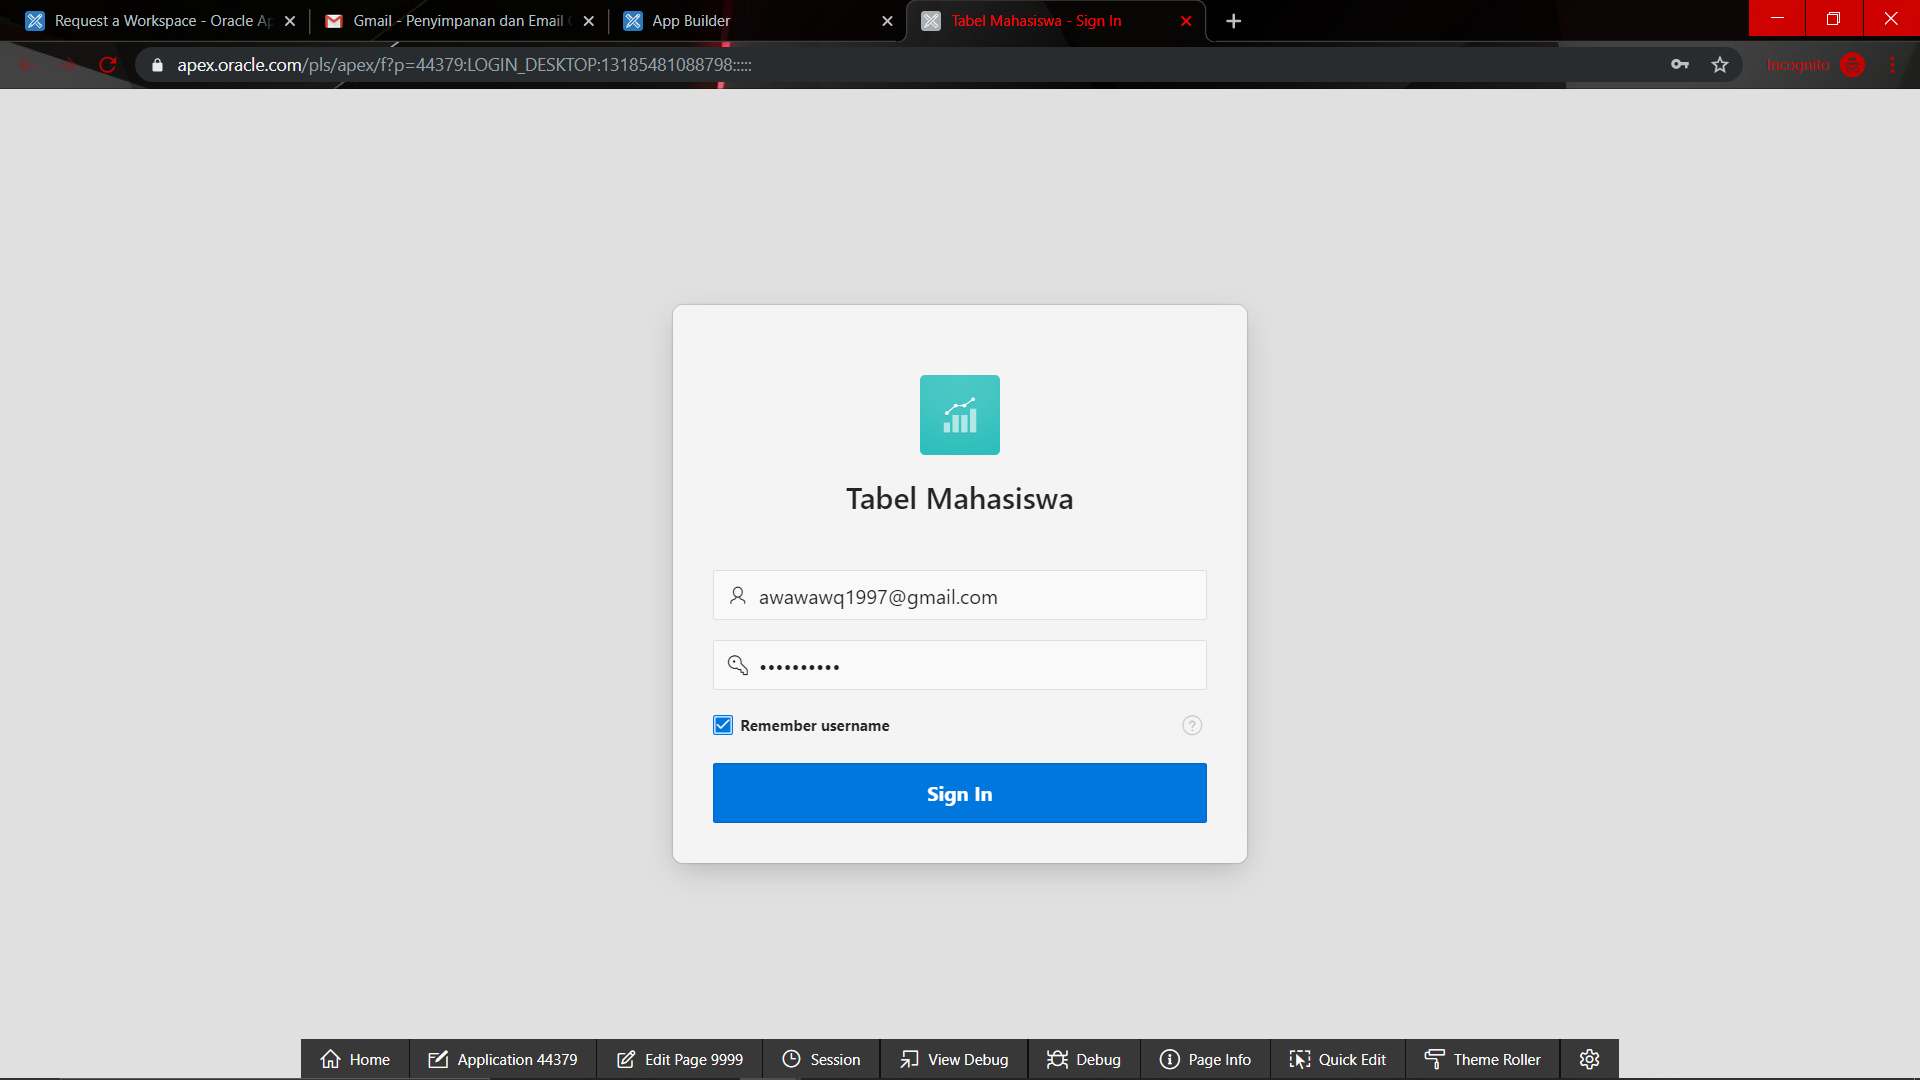
\includegraphics[scale=0.1]{figures/27}
    \caption{}
    \label{Variable Explorer}
\end{figure}



\item aplikasi apex sudah selesai dibuat
\begin{figure}[H]
    \centering
    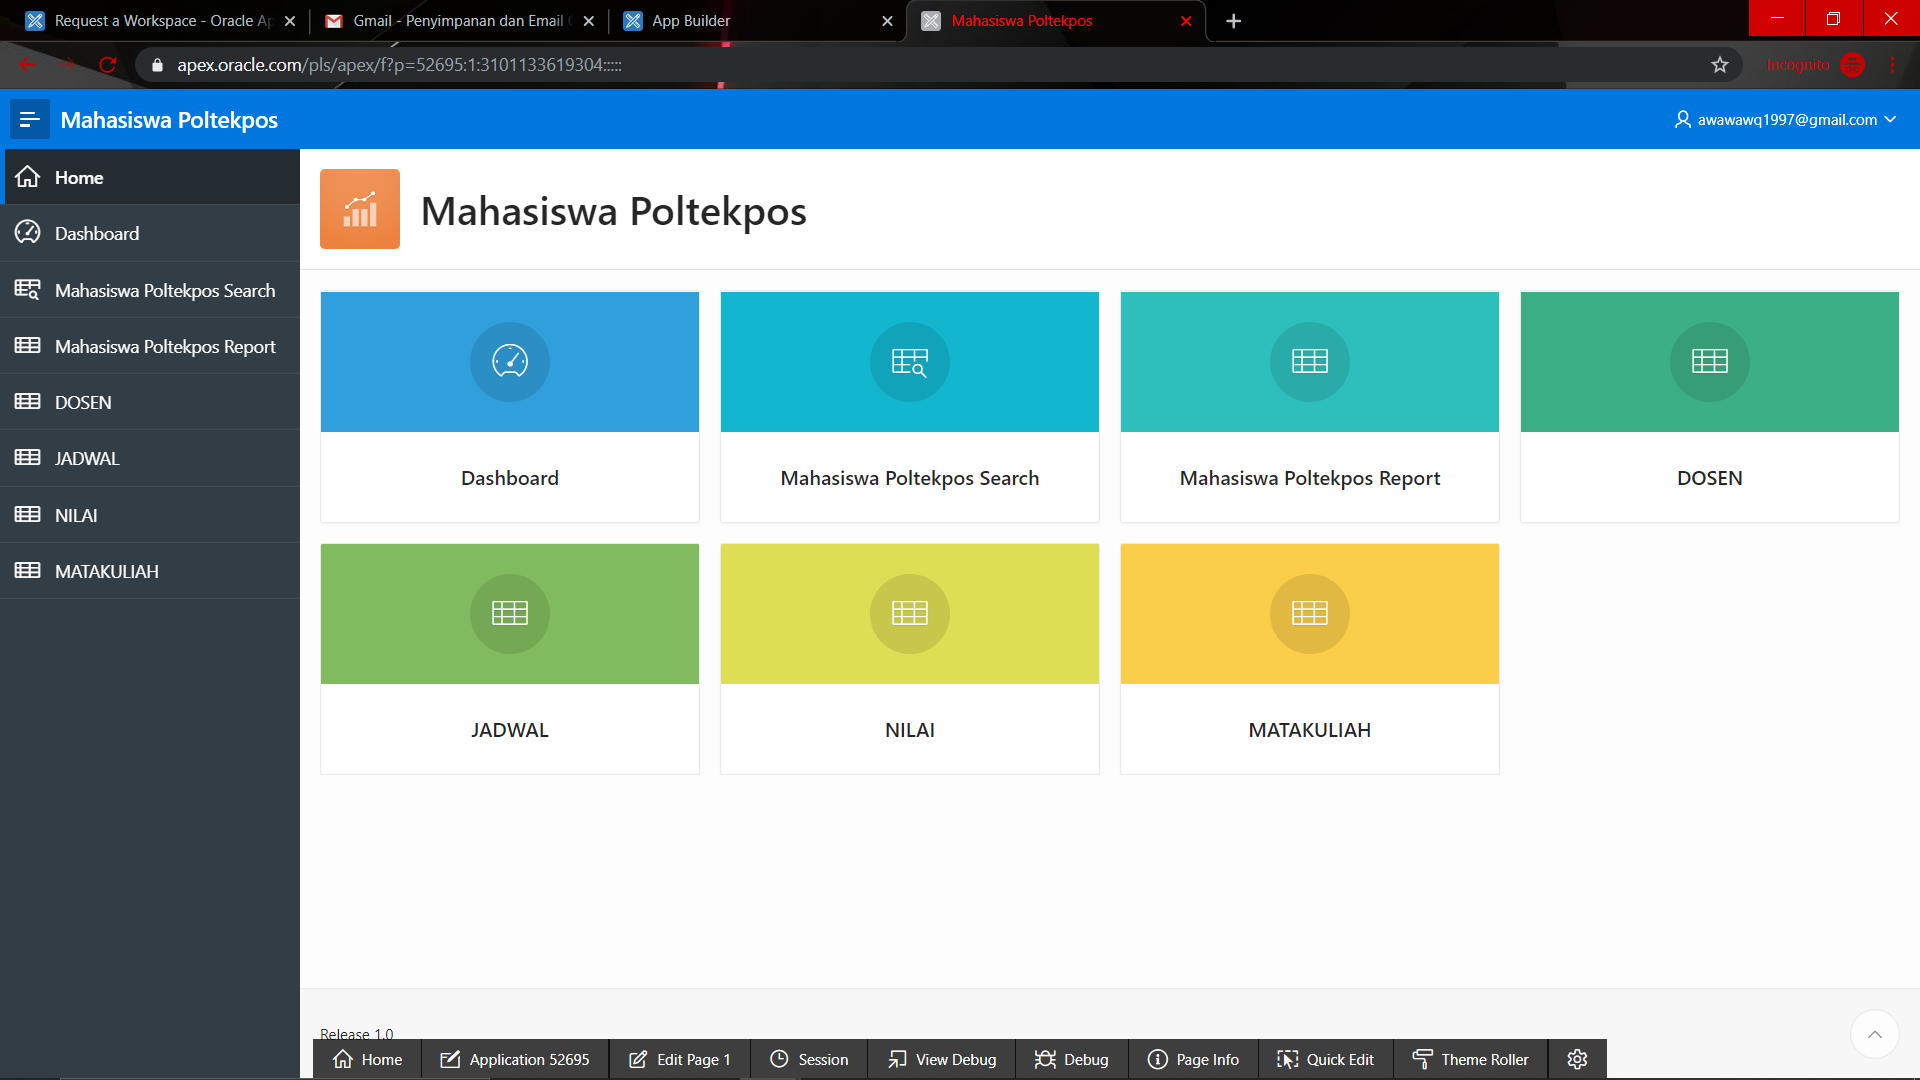
\includegraphics[scale=0.1]{figures/28}
    \caption{}
    \label{Indentasi}
\end{figure}
\end{enumerate}

\par 
Username : awawawq1997@gmail.com \\
Password : kinoyku123 \\
link     : https://apex.oracle.com/pls/apex/f?p=52695:1:35108638267405:::::
